% Vehicle Currency Rotation in Decentralised Exchanges
% Working-title contract: the current title states the route-composition finding that the
% manuscript actually establishes. A mechanism title requires completed cost, liquidity,
% risk, and architecture tests and must not be restored on the strength of designs alone.
%
% Architecture draws on docs/paper-spine.md, which derives the eventual full manuscript
% from nine JFE papers read first-hand. This working version contains the six sections
% supported by current evidence; it retains no standalone literature review or body proof.
%
% Section files are separate so they can be written and reviewed independently. Numbers
% come from output/exhibits/ and are never typed from memory; every one carries a comment
% naming the exhibit it was read from.
\documentclass[11pt]{article}

\usepackage[margin=1in]{geometry}
\usepackage{amsmath,amssymb}
\usepackage{booktabs}
\usepackage{array,tabularx}
\usepackage{graphicx}
\usepackage{tikz}
\usepackage{pgfplots}
\pgfplotsset{compat=1.18}
\usepackage{natbib}
\usepackage{setspace}
\usepackage{hyperref}
\usepackage{acro}
\usepackage[section]{placeins}
\hypersetup{colorlinks=true, linkcolor=[rgb]{0.05,0.25,0.65}, citecolor=[rgb]{0.05,0.25,0.65},
            urlcolor=[rgb]{0.05,0.25,0.65}, filecolor=[rgb]{0.05,0.25,0.65}}
\newcommand{\ethtx}[2]{\href{https://etherscan.io/tx/#1}{\texttt{#2}}}
\DeclareAcronym{amm}{short=AMM,long=automated market maker}

\bibliographystyle{chicago}
\onehalfspacing

% JFE-style exhibit treatment. Captions sit above the exhibit; notes use the full
% available line width and the surrounding prose alignment, with the journal's
% singular ``Note:'' label even when the note contains several sentences.
\setlength{\belowcaptionskip}{8pt}
\newcommand{\exhibitnote}[1]{%
  \par\vspace{6pt}%
  \noindent\begin{minipage}{\linewidth}%
    \footnotesize\emph{Note:} #1\par
  \end{minipage}%
}

% Certified route-only quantities shared with the live deck. The source file is
% regenerated from the findings registry; exact-state results remain excluded.
% Generated by scripts/tabulate/render_provisional_results_deck_values.py.
% PROVISIONAL working-paper values; scientific identity is recorded in the provenance sidecar.
\newcommand{\StableCountBase}{16.9\%}
\newcommand{\StableCountEnd}{42.3\%}
\newcommand{\StableCountChange}{$+25.4$ pp}
\newcommand{\StableCountSE}{1.05 pp}
\newcommand{\StableCountP}{$3.35\times10^{-87}$}
\newcommand{\StableValueBase}{32.7\%}
\newcommand{\StableValueEnd}{76.5\%}
\newcommand{\StableValueChange}{$+43.9$ pp}
\newcommand{\StableValueSE}{2.02 pp}
\newcommand{\StableValueP}{$4.46\times10^{-75}$}
\newcommand{\MultiLegCountBase}{44.5\%}
\newcommand{\MultiLegCountEnd}{60.7\%}
\newcommand{\MultiLegCountChange}{$+16.3$ pp}
\newcommand{\MultiLegCountSE}{1.86 pp}
\newcommand{\MultiLegValueBase}{47.3\%}
\newcommand{\MultiLegValueEnd}{83.2\%}
\newcommand{\MultiLegValueChange}{$+35.9$ pp}
\newcommand{\MultiLegValueSE}{1.68 pp}
\newcommand{\WeakestComplexityCountChange}{$+17.0$ pp}
\newcommand{\WeakestComplexityCountSE}{1.36 pp}
\newcommand{\WeakestComplexityValueChange}{$+25.6$ pp}
\newcommand{\WeakestComplexityValueSE}{1.52 pp}
\newcommand{\JointStableContribution}{92.1\%}
\newcommand{\USDTCountExcessBase}{1.06}
\newcommand{\USDTCountExcessEnd}{1.23}
\newcommand{\USDTValueExcessBase}{0.59}
\newcommand{\USDTValueExcessEnd}{1.42}
\newcommand{\USDTCrossCountChange}{$+7.59$ pp}
\newcommand{\USDTCrossCountSE}{0.88 pp}
\newcommand{\USDTCrossValueChange}{$+12.00$ pp}
\newcommand{\USDTCrossValueSE}{2.03 pp}
\newcommand{\USDTEndpointGapBase}{$-7.13$ pp}
\newcommand{\USDTEndpointGapEnd}{$+8.14$ pp}
\newcommand{\USDTEndpointGapChange}{$+15.27$ pp}
\newcommand{\USDTEndpointGapSE}{1.50 pp}
\newcommand{\FullIntermediationBase}{13.95\%}
\newcommand{\FullIntermediationEnd}{11.92\%}
\newcommand{\FullIntermediationChange}{$-2.03$ pp}
\newcommand{\FullIntermediationSE}{0.39 pp}
\newcommand{\BalancedIntermediationEnd}{8.60\%}
\newcommand{\BalancedIntermediationChange}{$-5.35$ pp}
\newcommand{\BalancedIntermediationSE}{0.38 pp}
\newcommand{\CrossVenueCountStart}{2.0\%}
\newcommand{\CrossVenueCountEnd}{57.2\%}
\newcommand{\CrossVenueValueEnd}{79.1\%}
\newcommand{\CrossVenueRotationPremium}{$+7.45$ pp}
\newcommand{\CrossVenueRotationSE}{1.33 pp}
\newcommand{\VenueAllStableCountBase}{1.27}
\newcommand{\VenueAllStableCountEnd}{1.41}
\newcommand{\VenueAllStableValueBase}{0.84}
\newcommand{\VenueAllStableValueEnd}{1.24}
\newcommand{\VenueCPStableCountBase}{1.28}
\newcommand{\VenueCPStableCountEnd}{1.42}
\newcommand{\VenueCPStableValueBase}{0.78}
\newcommand{\VenueCPStableValueEnd}{1.33}
\newcommand{\VenueCPNativeValueEnd}{0.62}
\newcommand{\VenueAllStableValueChange}{$+0.40$}
\newcommand{\VenueCPStableValueChange}{$+0.55$}
\newcommand{\VenueCPEpisodeShare}{84.8\%}
\newcommand{\VenueBalancerPeakEpisodes}{39,536}
\newcommand{\VenueCPPeakEpisodes}{8,767,213}
\newcommand{\RouterWindowDays}{60}
\newcommand{\RouterReleaseCount}{3}
\newcommand{\RouterIntermediationBase}{20.8\%}
\newcommand{\RouterIntermediationEnd}{12.5\%}
\newcommand{\RouterIntermediationOne}{$-5.7$ pp}
\newcommand{\RouterIntermediationTwo}{$+0.8$ pp}
\newcommand{\RouterIntermediationThree}{$-0.7$ pp}
\newcommand{\RouterLargestIntermediationRise}{$+0.8$ pp}
\newcommand{\RouterLargestLegMovement}{0.049}
\newcommand{\RouterCrossBase}{8.5\%}
\newcommand{\RouterCrossOne}{$+2.5$ pp}
\newcommand{\RouterCrossTwo}{$+3.1$ pp}
\newcommand{\RouterCrossThree}{$-2.0$ pp}
\newcommand{\RouterCrossEnd}{24.4\%}

% Generated by scripts/build_vehicle_transition_pair_deck_values.py; do not edit.
\newcommand{\PairPooledBase}{16.9\%}
\newcommand{\PairPooledEnd}{42.5\%}
\newcommand{\PairPooledTotal}{+25.7\,pp}
\newcommand{\PairPooledReweight}{+8.6\,pp}
\newcommand{\PairPooledSupportMass}{-0.5\,pp}
\newcommand{\PairPooledExclusive}{+17.8\,pp}
\newcommand{\PairPooledWithin}{-0.1\,pp}
\newcommand{\PairPooledBaseRawPct}{16.865562569}
\newcommand{\PairPooledEndRawPct}{42.540936227}
\newcommand{\PairPooledReweightRawPP}{8.572531324}
\newcommand{\PairPooledSupportMassRawPP}{-0.536299548}
\newcommand{\PairPooledExclusiveRawPP}{17.767073765}
\newcommand{\PairPooledWithinRawPP}{-0.127931883}
\newcommand{\PairSingleTotal}{+21.1\,pp}
\newcommand{\PairSingleWithin}{-0.3\,pp}
\newcommand{\PairCrossTotal}{+31.4\,pp}
\newcommand{\PairCrossWithin}{-0.3\,pp}
\newcommand{\PairValueTotal}{+42.8\,pp}
\newcommand{\PairValueWithin}{0.0\,pp}
\newcommand{\PairValueReweight}{+26.2\,pp}
\newcommand{\PairValueSupportMass}{-2.5\,pp}
\newcommand{\PairValueExclusive}{+19.2\,pp}

% Generated by scripts/process/build_v1_route_case.py; do not edit.
\newcommand{\VOneCaseDate}{15 March 2020}
\newcommand{\VOneCaseBlock}{9{,}674{,}728}
\newcommand{\VOneCaseEth}{439.13}
\newcommand{\VOneCaseTokenIn}{250}
\newcommand{\VOneCaseTokenOut}{49{,}892.40}
\newcommand{\VOneCaseSellExchange}{0x2c4bd0\ldots 0957}
\newcommand{\VOneCaseBuyExchange}{0x2a1530\ldots 8667}
\newcommand{\VOneCaseTx}{0x4dca160d762184835f34925a8cc556d7283a7642c88d1bef3382a73596a0ca16}
\newcommand{\VOneCaseTxShort}{0x4dca160d\ldots 96a0ca16}
\newcommand{\VOneCaseExactCount}{129{,}810}

% Dated backing regimes inside the stablecoin class. Provisional/E0 scope: the
% cut runs on the released endpoint-candidate choice panel and is not
% submission-authoritative until the findings freeze admits it. Refresh with
% scripts/run_vehicle_transition_e0.py then
% scripts/build_backing_regime_deck_values.py.
% Generated by scripts/build_backing_regime_deck_values.py.
% Dated backing regimes inside the stablecoin class, on the exact two-leg
% sample and the native-plus-stable denominator of the rotation. Provisional/E0
% scope: the estimates run on the released endpoint-candidate choice panel and
% are not submission-authoritative until the findings freeze admits them.
% Refresh by rerunning scripts/run_vehicle_transition_e0.py then this builder.
\newcommand{\BackingFiatCountChange}{$+24.50$ pp}
\newcommand{\BackingFiatCountSE}{1.08 pp}
\newcommand{\BackingFiatCountBase}{15.66\%}
\newcommand{\BackingFiatCountEnd}{40.16\%}
\newcommand{\BackingFiatCountMassBase}{93.1\%}
\newcommand{\BackingFiatCountMassEnd}{95.2\%}
\newcommand{\BackingSyntheticCountChange}{$+0.55$ pp}
\newcommand{\BackingSyntheticCountSE}{0.08 pp}
\newcommand{\BackingSyntheticCountBase}{0.04\%}
\newcommand{\BackingSyntheticCountEnd}{0.60\%}
\newcommand{\BackingSyntheticCountMassBase}{0.3\%}
\newcommand{\BackingSyntheticCountMassEnd}{1.4\%}
\newcommand{\BackingOnChainCountChange}{$+0.23$ pp}
\newcommand{\BackingOnChainCountSE}{0.09 pp}
\newcommand{\BackingOnChainCountBase}{0.03\%}
\newcommand{\BackingOnChainCountEnd}{0.26\%}
\newcommand{\BackingOnChainCountMassBase}{0.2\%}
\newcommand{\BackingOnChainCountMassEnd}{0.6\%}
\newcommand{\BackingRwaCountChange}{$+0.00$ pp}
\newcommand{\BackingRwaCountSE}{0.21 pp}
\newcommand{\BackingRwaCountBase}{1.05\%}
\newcommand{\BackingRwaCountEnd}{1.05\%}
\newcommand{\BackingRwaCountMassBase}{5.8\%}
\newcommand{\BackingRwaCountMassEnd}{2.4\%}
\newcommand{\BackingNonUsdCountChange}{$+0.01$ pp}
\newcommand{\BackingNonUsdCountSE}{0.03 pp}
\newcommand{\BackingNonUsdCountBase}{0.07\%}
\newcommand{\BackingNonUsdCountEnd}{0.08\%}
\newcommand{\BackingNonUsdCountMassBase}{0.4\%}
\newcommand{\BackingNonUsdCountMassEnd}{0.2\%}
\newcommand{\BackingFraxTransitionCountChange}{$+0.12$ pp}
\newcommand{\BackingFraxTransitionCountSE}{0.03 pp}
\newcommand{\BackingFraxTransitionCountBase}{0.03\%}
\newcommand{\BackingFraxTransitionCountEnd}{0.15\%}
\newcommand{\BackingFraxTransitionCountMassBase}{0.2\%}
\newcommand{\BackingFraxTransitionCountMassEnd}{0.3\%}
\newcommand{\BackingPooledCountChange}{$+25.42$ pp}
\newcommand{\BackingPooledCountSE}{1.05 pp}
\newcommand{\BackingPooledCountBase}{16.89\%}
\newcommand{\BackingPooledCountEnd}{42.31\%}
\newcommand{\BackingPooledCountMassBase}{100.0\%}
\newcommand{\BackingPooledCountMassEnd}{100.0\%}
\newcommand{\BackingCountUniverseGap}{0.001 pp}
\newcommand{\BackingFiatValueChange}{$+44.09$ pp}
\newcommand{\BackingFiatValueSE}{2.07 pp}
\newcommand{\BackingFiatValueBase}{28.86\%}
\newcommand{\BackingFiatValueEnd}{72.95\%}
\newcommand{\BackingFiatValueMassBase}{89.1\%}
\newcommand{\BackingFiatValueMassEnd}{95.4\%}
\newcommand{\BackingSyntheticValueChange}{$+1.66$ pp}
\newcommand{\BackingSyntheticValueSE}{0.50 pp}
\newcommand{\BackingSyntheticValueBase}{0.86\%}
\newcommand{\BackingSyntheticValueEnd}{2.53\%}
\newcommand{\BackingSyntheticValueMassBase}{3.0\%}
\newcommand{\BackingSyntheticValueMassEnd}{3.0\%}
\newcommand{\BackingOnChainValueChange}{$+0.12$ pp}
\newcommand{\BackingOnChainValueSE}{0.13 pp}
\newcommand{\BackingOnChainValueBase}{0.10\%}
\newcommand{\BackingOnChainValueEnd}{0.22\%}
\newcommand{\BackingOnChainValueMassBase}{0.2\%}
\newcommand{\BackingOnChainValueMassEnd}{0.2\%}
\newcommand{\BackingRwaValueChange}{$-1.73$ pp}
\newcommand{\BackingRwaValueSE}{0.44 pp}
\newcommand{\BackingRwaValueBase}{2.54\%}
\newcommand{\BackingRwaValueEnd}{0.81\%}
\newcommand{\BackingRwaValueMassBase}{6.8\%}
\newcommand{\BackingRwaValueMassEnd}{1.4\%}
\newcommand{\BackingNonUsdValueChange}{$-0.18$ pp}
\newcommand{\BackingNonUsdValueSE}{0.08 pp}
\newcommand{\BackingNonUsdValueBase}{0.19\%}
\newcommand{\BackingNonUsdValueEnd}{0.00\%}
\newcommand{\BackingNonUsdValueMassBase}{0.5\%}
\newcommand{\BackingNonUsdValueMassEnd}{0.0\%}
\newcommand{\BackingFraxTransitionValueChange}{$-0.09$ pp}
\newcommand{\BackingFraxTransitionValueSE}{0.02 pp}
\newcommand{\BackingFraxTransitionValueBase}{0.10\%}
\newcommand{\BackingFraxTransitionValueEnd}{0.02\%}
\newcommand{\BackingFraxTransitionValueMassBase}{0.3\%}
\newcommand{\BackingFraxTransitionValueMassEnd}{0.0\%}
\newcommand{\BackingPooledValueChange}{$+43.87$ pp}
\newcommand{\BackingPooledValueSE}{2.02 pp}
\newcommand{\BackingPooledValueBase}{32.66\%}
\newcommand{\BackingPooledValueEnd}{76.53\%}
\newcommand{\BackingPooledValueMassBase}{100.0\%}
\newcommand{\BackingPooledValueMassEnd}{100.0\%}
\newcommand{\BackingValueUniverseGap}{0.000 pp}
\newcommand{\BackingCandidates}{21}
\newcommand{\BackingLabelMovesInWindow}{0}
\newcommand{\BackingLabelMovesInPanel}{2}

% Fixed-cohort conditioning of the rotation. Provisional/E0 scope: the cohorts
% run on the released endpoint-candidate choice panel and are not
% submission-authoritative until the findings freeze admits them. A conditional
% macro is the change among cells active in both endpoint years, so it is only
% ever spent beside its own retained-mass macro. Refresh with
% scripts/run_vehicle_transition_e0.py then
% scripts/build_fixed_opportunity_deck_values.py.
% Generated by scripts/build_fixed_opportunity_deck_values.py.
% Fixed-cohort conditioning of the vehicle rotation, on the exact two-leg
% sample and the native-plus-stable denominator. Provisional/E0 scope: the
% estimates run on the released endpoint-candidate choice panel and are not
% submission-authoritative until the findings freeze admits them.
% Cohort membership is decided using both endpoint years, so a conditional
% row is the change among continuously active cells, not the full-universe
% change; always spend it beside its retained-mass macro.
% Refresh by rerunning scripts/run_vehicle_transition_e0.py then this builder.
\newcommand{\FixedPooledCountChange}{$+25.42$ pp}
\newcommand{\FixedPooledCountSE}{1.05 pp}
\newcommand{\FixedPooledCountCILower}{$+23.35$ pp}
\newcommand{\FixedPooledCountCIUpper}{$+27.48$ pp}
\newcommand{\FixedPooledCountBase}{16.89\%}
\newcommand{\FixedPooledCountEnd}{42.31\%}
\newcommand{\FixedPairCountChange}{$+14.85$ pp}
\newcommand{\FixedPairCountSE}{1.02 pp}
\newcommand{\FixedPairCountCILower}{$+12.85$ pp}
\newcommand{\FixedPairCountCIUpper}{$+16.86$ pp}
\newcommand{\FixedPairCountBase}{24.76\%}
\newcommand{\FixedPairCountEnd}{39.62\%}
\newcommand{\FixedPairCountMassBase}{55.5\%}
\newcommand{\FixedPairCountMassEnd}{57.7\%}
\newcommand{\FixedCandidateCountChange}{$+12.94$ pp}
\newcommand{\FixedCandidateCountSE}{0.94 pp}
\newcommand{\FixedCandidateCountCILower}{$+11.10$ pp}
\newcommand{\FixedCandidateCountCIUpper}{$+14.78$ pp}
\newcommand{\FixedCandidateCountBase}{23.41\%}
\newcommand{\FixedCandidateCountEnd}{36.34\%}
\newcommand{\FixedCandidateCountMassBase}{54.0\%}
\newcommand{\FixedCandidateCountMassEnd}{54.6\%}
\newcommand{\FixedVenueCountChange}{$-0.18$ pp}
\newcommand{\FixedVenueCountSE}{0.99 pp}
\newcommand{\FixedVenueCountCILower}{$-2.13$ pp}
\newcommand{\FixedVenueCountCIUpper}{$+1.76$ pp}
\newcommand{\FixedVenueCountBase}{24.47\%}
\newcommand{\FixedVenueCountEnd}{24.29\%}
\newcommand{\FixedVenueCountMassBase}{45.5\%}
\newcommand{\FixedVenueCountMassEnd}{38.9\%}
\newcommand{\FixedCountUniverseGap}{0.001 pp}
\newcommand{\FixedPooledValueChange}{$+43.87$ pp}
\newcommand{\FixedPooledValueSE}{2.02 pp}
\newcommand{\FixedPooledValueCILower}{$+39.91$ pp}
\newcommand{\FixedPooledValueCIUpper}{$+47.84$ pp}
\newcommand{\FixedPooledValueBase}{32.66\%}
\newcommand{\FixedPooledValueEnd}{76.53\%}
\newcommand{\FixedPairValueChange}{$+39.36$ pp}
\newcommand{\FixedPairValueSE}{2.18 pp}
\newcommand{\FixedPairValueCILower}{$+35.07$ pp}
\newcommand{\FixedPairValueCIUpper}{$+43.64$ pp}
\newcommand{\FixedPairValueBase}{37.55\%}
\newcommand{\FixedPairValueEnd}{76.91\%}
\newcommand{\FixedPairValueMassBase}{82.2\%}
\newcommand{\FixedPairValueMassEnd}{77.1\%}
\newcommand{\FixedCandidateValueChange}{$+37.24$ pp}
\newcommand{\FixedCandidateValueSE}{1.86 pp}
\newcommand{\FixedCandidateValueCILower}{$+33.59$ pp}
\newcommand{\FixedCandidateValueCIUpper}{$+40.89$ pp}
\newcommand{\FixedCandidateValueBase}{36.64\%}
\newcommand{\FixedCandidateValueEnd}{73.88\%}
\newcommand{\FixedCandidateValueMassBase}{80.4\%}
\newcommand{\FixedCandidateValueMassEnd}{66.1\%}
\newcommand{\FixedVenueValueChange}{$+21.74$ pp}
\newcommand{\FixedVenueValueSE}{2.46 pp}
\newcommand{\FixedVenueValueCILower}{$+16.91$ pp}
\newcommand{\FixedVenueValueCIUpper}{$+26.57$ pp}
\newcommand{\FixedVenueValueBase}{36.74\%}
\newcommand{\FixedVenueValueEnd}{58.48\%}
\newcommand{\FixedVenueValueMassBase}{73.3\%}
\newcommand{\FixedVenueValueMassEnd}{37.3\%}
\newcommand{\FixedValueUniverseGap}{0.000 pp}
\newcommand{\FixedPairCells}{39,748}
\newcommand{\FixedPairUniverseCells}{1,273,105}
\newcommand{\FixedCandidateCells}{40,368}
\newcommand{\FixedCandidateUniverseCells}{1,285,022}
\newcommand{\FixedVenueCells}{42,772}
\newcommand{\FixedVenueUniverseCells}{1,481,816}
\newcommand{\FixedUnsupportedDimensions}{3}
\newcommand{\FixedCohortDays}{543}

% Within-day cross-section of the excess-use construct. Provisional/E0 scope: the
% ladder runs on the green route-only D3 panel and is not submission-authoritative
% until the findings freeze admits it. Refresh with
% scripts/run_excess_use_date_fe_ladder.py then
% scripts/build_excess_use_date_fe_deck_values.py.
% Generated by scripts/build_excess_use_date_fe_deck_values.py.
% Within-day cross-section of the excess-use construct: token-day intermediary
% count share on own endpoint count share, both in percentage points, date
% fixed effects absorbing the calendar. Provisional/E0 scope: the estimates run
% on the green route-only D3 panel and are not submission-authoritative until
% the findings freeze admits them. Refresh by rerunning
% scripts/run_excess_use_date_fe_ladder.py then this builder.
\newcommand{\DateFEPooledNative}{$+34.56$ pp}
\newcommand{\DateFEPooledNativeSE}{23.04 pp}
\newcommand{\DateFEPooledNativeCI}{$[-10.62, +79.75]$}
\newcommand{\DateFEPooledNativeP}{$p = 0.134$}
\newcommand{\DateFEPooledStable}{$+2.42$ pp}
\newcommand{\DateFEPooledStableSE}{1.32 pp}
\newcommand{\DateFEPooledStableCI}{$[-0.17, +5.01]$}
\newcommand{\DateFEPooledStableP}{$p = 0.067$}
\newcommand{\DateFEDayNative}{$+34.55$ pp}
\newcommand{\DateFEDayNativeSE}{23.04 pp}
\newcommand{\DateFEDayNativeCI}{$[-10.64, +79.74]$}
\newcommand{\DateFEDayNativeP}{$p = 0.134$}
\newcommand{\DateFEDayStable}{$+2.42$ pp}
\newcommand{\DateFEDayStableSE}{1.32 pp}
\newcommand{\DateFEDayStableCI}{$[-0.17, +5.01]$}
\newcommand{\DateFEDayStableP}{$p = 0.067$}
\newcommand{\DateFEDemandNative}{$+0.05$ pp}
\newcommand{\DateFEDemandNativeSE}{0.56 pp}
\newcommand{\DateFEDemandNativeCI}{$[-1.04, +1.14]$}
\newcommand{\DateFEDemandNativeP}{$p = 0.924$}
\newcommand{\DateFEDemandStable}{$+0.85$ pp}
\newcommand{\DateFEDemandStableSE}{0.50 pp}
\newcommand{\DateFEDemandStableCI}{$[-0.13, +1.83]$}
\newcommand{\DateFEDemandStableP}{$p = 0.090$}
\newcommand{\DateFEDemandImported}{$+0.14$ pp}
\newcommand{\DateFEDemandImportedSE}{0.11 pp}
\newcommand{\DateFEDemandImportedCI}{$[-0.08, +0.35]$}
\newcommand{\DateFEDemandImportedP}{$p = 0.207$}
\newcommand{\DateFEDemandStaked}{$+0.12$ pp}
\newcommand{\DateFEDemandStakedSE}{0.07 pp}
\newcommand{\DateFEDemandStakedCI}{$[-0.03, +0.26]$}
\newcommand{\DateFEDemandStakedP}{$p = 0.108$}
\newcommand{\DateFESlope}{1.587}
\newcommand{\DateFESlopeSE}{0.026}
\newcommand{\DateFESlopeCI}{$[+1.54, +1.64]$}
\newcommand{\DateFESlopeP}{$p < 0.001$}
\newcommand{\DateFESlopeWithinToken}{0.985}
\newcommand{\DateFESlopeWithinTokenSE}{0.301}
\newcommand{\DateFESlopeWithinTokenCI}{$[+0.39, +1.57]$}
\newcommand{\DateFESlopeWithinTokenP}{$p = 0.001$}
\newcommand{\DateFEStableMinusNative}{$+0.79$ pp}
\newcommand{\DateFEStableMinusNativeSE}{1.02 pp}
\newcommand{\DateFEStableMinusNativeCI}{$[-1.20, +2.78]$}
\newcommand{\DateFEStableMinusNativeP}{$p = 0.435$}
\newcommand{\DateFESlopeStableMinusNative}{0.351}
\newcommand{\DateFESlopeStableMinusNativeSE}{0.263}
\newcommand{\DateFESlopeStableMinusNativeCI}{$[-0.17, +0.87]$}
\newcommand{\DateFESlopeStableMinusNativeP}{$p = 0.183$}
\newcommand{\DateFESlopeNativeMinusImported}{0.075}
\newcommand{\DateFESlopeNativeMinusImportedSE}{0.028}
\newcommand{\DateFESlopeNativeMinusImportedCI}{$[+0.02, +0.13]$}
\newcommand{\DateFESlopeNativeMinusImportedP}{$p = 0.007$}
\newcommand{\DateFEWeightedNative}{$-15.91$ pp}
\newcommand{\DateFEWeightedNativeSE}{8.08 pp}
\newcommand{\DateFEWeightedNativeCI}{$[-31.76, -0.07]$}
\newcommand{\DateFEWeightedNativeP}{$p = 0.049$}
\newcommand{\DateFEWeightedSlope}{2.012}
\newcommand{\DateFEWeightedSlopeSE}{0.197}
\newcommand{\DateFEWeightedSlopeCI}{$[+1.63, +2.40]$}
\newcommand{\DateFEWeightedSlopeP}{$p < 0.001$}
\newcommand{\DateFECandidateNative}{$-17.45$ pp}
\newcommand{\DateFECandidateNativeSE}{7.63 pp}
\newcommand{\DateFECandidateNativeCI}{$[-32.41, -2.49]$}
\newcommand{\DateFECandidateNativeP}{$p = 0.022$}
\newcommand{\DateFECandidateImported}{$-1.34$ pp}
\newcommand{\DateFECandidateImportedSE}{0.62 pp}
\newcommand{\DateFECandidateImportedCI}{$[-2.55, -0.13]$}
\newcommand{\DateFECandidateImportedP}{$p = 0.030$}
\newcommand{\DateFEClassifiedNative}{$-1.51$ pp}
\newcommand{\DateFEClassifiedNativeSE}{1.27 pp}
\newcommand{\DateFEClassifiedNativeCI}{$[-4.09, +1.06]$}
\newcommand{\DateFEClassifiedNativeP}{$p = 0.240$}
\newcommand{\DateFEClassifiedImported}{$-0.64$ pp}
\newcommand{\DateFEClassifiedImportedSE}{0.48 pp}
\newcommand{\DateFEClassifiedImportedCI}{$[-1.62, +0.34]$}
\newcommand{\DateFEClassifiedImportedP}{$p = 0.192$}
\newcommand{\DateFEBackingOnChain}{$-0.77$ pp}
\newcommand{\DateFEBackingOnChainSE}{0.29 pp}
\newcommand{\DateFEBackingOnChainCI}{$[-1.35, -0.20]$}
\newcommand{\DateFEBackingOnChainP}{$p = 0.008$}
\newcommand{\DateFEBackingSynthetic}{$-0.61$ pp}
\newcommand{\DateFEBackingSyntheticSE}{0.26 pp}
\newcommand{\DateFEBackingSyntheticCI}{$[-1.11, -0.11]$}
\newcommand{\DateFEBackingSyntheticP}{$p = 0.017$}
\newcommand{\DateFEBackingRWA}{$-0.50$ pp}
\newcommand{\DateFEBackingRWASE}{0.33 pp}
\newcommand{\DateFEBackingRWACI}{$[-1.14, +0.14]$}
\newcommand{\DateFEBackingRWAP}{$p = 0.125$}
\newcommand{\DateFETether}{$-5.32$ pp}
\newcommand{\DateFETetherSE}{0.93 pp}
\newcommand{\DateFETetherCI}{$[-7.14, -3.51]$}
\newcommand{\DateFETetherP}{$p < 0.001$}
\newcommand{\DateFESlopeEarly}{1.605}
\newcommand{\DateFESlopeEarlySE}{0.034}
\newcommand{\DateFESlopeEarlyCI}{$[+1.54, +1.67]$}
\newcommand{\DateFESlopeEarlyP}{$p < 0.001$}
\newcommand{\DateFESlopeLate}{1.554}
\newcommand{\DateFESlopeLateSE}{0.026}
\newcommand{\DateFESlopeLateCI}{$[+1.50, +1.60]$}
\newcommand{\DateFESlopeLateP}{$p < 0.001$}
\newcommand{\DateFENativeEarly}{$+0.70$ pp}
\newcommand{\DateFENativeEarlySE}{0.98 pp}
\newcommand{\DateFENativeEarlyCI}{$[-1.22, +2.63]$}
\newcommand{\DateFENativeEarlyP}{$p = 0.473$}
\newcommand{\DateFENativeLate}{$-0.72$ pp}
\newcommand{\DateFENativeLateSE}{0.94 pp}
\newcommand{\DateFENativeLateCI}{$[-2.56, +1.12]$}
\newcommand{\DateFENativeLateP}{$p = 0.441$}
\newcommand{\DateFETokenDays}{1,828,862}
\newcommand{\DateFETokens}{304,572}
\newcommand{\DateFEDays}{2,259}
\newcommand{\DateFEAbsorbedDays}{2,259}
\newcommand{\DateFEWithinTokenAbsorbed}{306,830}
\newcommand{\DateFECandidateTokenDays}{11,233}
\newcommand{\DateFECandidateDays}{2,258}
\newcommand{\DateFEClassifiedTokenDays}{44,077}
\newcommand{\DateFEClassifiedTokens}{37}
\newcommand{\DateFECeilingMean}{0.0008}
\newcommand{\DateFECeilingNinetyNinth}{0.0004}
\newcommand{\DateFECeilingHalfShare}{0.08\%}
\newcommand{\DateFELeaveOutSlope}{3.209}
\newcommand{\DateFELeaveOutSlopeSE}{0.090}
\newcommand{\DateFEFloorFiveSlope}{1.579}
\newcommand{\DateFEFloorHundredSlope}{1.595}


\title{Vehicle Currency Rotation in Decentralised Exchanges}
% Author list intentionally withheld until coauthorship is settled.
% \author{Jiahua Xu\thanks{University College London, Centre for Blockchain Technologies.}}
\author{}
\date{\today}

\begin{document}

\maketitle

\begin{abstract}
% Working-paper abstract: update whenever a substantive result changes.
We reconstruct \RoutePanelRawSwaps{} swaps and observe the vehicle inside each connected route. From 2024 H1 to 2026 H1, stablecoin share rises 25.5 percentage points (pp). Net switching within continuing pairs is \PairPooledWithin{}, while pairs first observed after 2024 H1 contribute \PairLifecycleCountEntry{}. The entry vehicle predicts subsequent use. At the first sampled exact contest, it carries \FirstContestRouteRetention{} of routes and current output predicts retention. When exact-output leadership changes hands, route share follows; prior weak-leg capital predicts whether the new lead persists. Dominance therefore shifts mainly through pair formation and activity reallocation, while prices and two-leg depth sustain vehicles inside established pairs.

\end{abstract}

% Section 1. Introduction.
% Status: first publication-standard rewrite against docs/findings-freeze.md.
% Admitted here: route-only vehicle rotation, excess use, and integration strata.
% Excluded: retired direct-route incidence, preliminary 1.17 hazard, LP returns,
% cross-venue spillover interpretation, and all final cost/persistence inference.

\section{Introduction}
\label{sec:intro}

A vehicle currency is traded not because it is one side of the desired payment, but because it is the market's preferred way to move between two other currencies. This role is highly concentrated in foreign exchange. Theories of vehicle currencies attribute that concentration to a feedback between use and transaction cost: routing more trades through one currency deepens its markets, and deeper markets make it attractive to route still more trades through it \citep{Krugman1980VehicleCurrencies}. Monetary-search models generate a related coordination force because accepting an intermediary object is valuable when others are expected to accept it later \citep{KiyotakiWright1989MoneyMedium}. Related models show how the same coordination forces can sustain a currency's role in invoicing, funding, and balance sheets \citep{GopinathEtAl2020DCP,GopinathStein2021Making,Mukhin2022InternationalPriceSystem}.

The empirical obstacle is that the vehicle route is usually latent. Foreign-exchange records reveal turnover and prices while leaving the market-wide path of a payment and its feasible alternatives unobserved. A currency's international role can therefore be measured by the number of markets quoting it \citep{FlandreauJobst2009Empirics}, or inferred from price and volume responses \citep{Somogyi2026DollarDominanceFX}; realised intermediary use on individual routes remains hidden. This makes the central transition difficult to study. A dominant currency can lose transaction share without losing its intermediary role, and a new currency can gain endpoint demand without becoming the object others trade through.

This paper measures that role in decentralised exchange. A swap transaction records an ordered path through a graph of automated markets. When a route exchanges asset $i$ for asset $o$ through asset $k$, the intermediary is observed directly. The same record identifies the endpoints, so vehicle use can be separated from ordinary demand for $k$ as a source or destination. The setting also follows one currency system from an architecture that required native-asset intermediation to designs in which arbitrary pairs and competing routes are available. That history makes vehicle choice observable. Protocol launches coincide with other market changes, so their dates provide chronology but fail as treatments.

The primary unit is an exact two-leg route, which gives each realised vehicle choice one intermediary and one vote. Vehicle dominance is the share of these choices carried by an asset or asset class. I also construct a vehicle excess-use ratio: an asset's intermediary share divided by its endpoint share on the same route perimeter. A value above one means that the asset's intermediary share exceeds its endpoint share. This distinction is important in a market where stablecoins can become popular endpoints at the same time that they become useful bridges between other assets.

Stablecoins gain sharply as vehicle currencies, although the change is not steady. On calendar days observed in both endpoint years, their equal-weighted share among native and stable vehicles rises from \StableCountBase{} in 2024 to \StableCountEnd{} in 2026, a \StableCountChange{} change with a calendar-HAC standard error of \StableCountSE{}. On value supported within 20\% of route input, the corresponding share rises from \StableValueBase{} to \StableValueEnd{}, a \StableValueChange{} change with a standard error of \StableValueSE{}. Native intermediation rebounds in 2023 and 2024; stablecoins recover the value lead in 2025, while their lead by route count remains short-lived. I therefore describe the episode as a rotation. Persistent replacement would require a longer post-change lead.
% docs/findings-freeze.md, vehicle-dominance claim; exact two-leg unit

An aggregate share leaves open whether stablecoins replace the native asset on the same endpoint pairs or gain as routed activity moves across pairs. I distinguish these cases with a five-term accounting of pooled route count, whose stable share rises from \MarketBridgeBase{} to \MarketBridgeEnd{}. Pairs represented in the admitted route-component ledger in only one endpoint year contribute \MarketSupportBridge{} of the \MarketBridgeTotal{} increase. Among pairs represented in both endpoint years, differences in whether a native-or-stable vehicle route appears contribute \VehicleRoleSupportBridge{}. For pairs carrying these vehicle routes in both years, changes in their shares of admitted route-component activity contribute \MarketActivityReweight{}, changes in realised vehicle incidence contribute \VehicleIncidenceReweight{}, and changes in stable share contribute \WithinPairStableShare{}. Only the last term measures stable-for-native substitution within pairs carrying the vehicle role in both years. Most of the observed increase accompanies changes in pair representation, activity, and vehicle use.
% output/exhibits/vehicle_transition_pair_decomposition.jsonl; producer e16796c; evidence commit 23ee3a2

The stablecoin category also conceals an important difference between USDC and USDT. Together they account for \JointStableContribution{} of the increase in stable count share, but USDC begins the comparison with disproportionate vehicle use and changes little. USDT's count excess-use ratio rises from \USDTCountExcessBase{} to \USDTCountExcessEnd{}, while its strict-value ratio rises from \USDTValueExcessBase{} to \USDTValueExcessEnd{}. Its strict-value intermediary-minus-endpoint share moves from \USDTEndpointGapBase{} to \USDTEndpointGapEnd{}. USDT thus becomes more prominent in the intermediary position even relative to its use as an endpoint. The present comparisons do not distinguish among its backing, redemption, liquidity, and venue-reach features.
% docs/findings-freeze.md, token decomposition and excess-use transition

A widening trading network could produce these changes without a stronger coordination role for stablecoins. Cross-venue execution expands rapidly over the sample, yet the share of economic routes using a true intermediary falls from \FullIntermediationBase{} in 2022 to \FullIntermediationEnd{} in 2026 on the full perimeter and to \BalancedIntermediationEnd{} on a balanced five-venue perimeter. Among routes that remain indirect, stablecoin share rises in every observed integration-by-complexity count cell and rises \CrossVenueRotationPremium{} more across venues than within one venue, with a standard error of \CrossVenueRotationSE{}. Changes in broad route types therefore cannot account for the entire rotation. These comparisons do not hold fixed the endpoint pair, trade size, feasible paths, or router's decision state, so better search and changing venue reach remain viable explanations.
% output/exhibits/cross_venue_routing_inference.jsonl;
% docs/findings-freeze.md, integration-by-complexity and paired-date interaction

Protocol launches do not supply the missing fixed comparison. Entry and exit windows alter the set of observed routes, and role appearance or disappearance can coincide mechanically with the event window. I use these dates to describe chronology and do not treat them as estimates of an architecture effect.
% output/exhibits/architecture_transition_support.jsonl;
% output/exhibits/architecture_role_margin_support.jsonl

The paper makes three contributions. First, it observes the vehicle on each realised route and therefore separates vehicle status, which is binary on a route, from vehicle dominance, which is a continuous market share. The distinction turns the making of a vehicle currency from a quotation or aggregate-turnover object into a sequence of realised intermediary choices.

Second, the vehicle excess-use ratio benchmarks an asset's intermediary share against its observed endpoint share on the same route perimeter. It therefore distinguishes growth in ordinary stablecoin use from disproportionate use between other assets without requiring an exclusion restriction or a structural model.

Third, the paper distinguishes a change in vehicle choice within an endpoint pair from changes in which pairs carry vehicle routes, how much admitted route-component activity they receive, and how often that activity uses an intermediary. This distinction links aggregate vehicle dominance to the cross-section of routed markets instead of treating it as the choice of a representative pair.

The remainder of the paper proceeds as follows. Section~\ref{sec:setting} defines routes, vehicle dominance, and the data perimeter. Section~\ref{sec:dominance} measures the rotation and vehicle excess use. Section~\ref{sec:survival} defines persistence and the data required to estimate turnover. Section~\ref{sec:rivals} evaluates routing integration and the competing mechanisms. Section~\ref{sec:executability} describes exact-state reconstruction and the support required for counterfactual route costs. Section~\ref{sec:conclusion} concludes.

% Section 2. Institutional setting, definitions, and data.
%
% Every number here is read from an exhibit under output/exhibits/ or from a docs/finding-*
% file, and the comment above each one names the source. Nothing in this section is typed
% from memory. Six of nine JFE empirical papers read for this project make no causal claim
% and substitute a data moat plus a validation apparatus, so this section carries weight
% the identification strategy does not.

\section{Setting and data}
\label{sec:setting}

\subsection{Routes and notation}
\label{sec:setting:route}

In a limit order book, traders supply liquidity by posting orders at chosen prices. An \ac{amm} instead holds tokens in a pool and quotes mechanically against the pool's current state. Liquidity providers fund the pool, and a smart contract executes trades according to the protocol's pricing rule. \citet{LeharParlour2024Uniswap} describe the constant-product design and the economics of liquidity supply in these markets.

Multiple pools turn an exchange between two assets into a routing problem. A trader may use one pool, divide an order across pools, or trade through an intermediary asset. Routers compare and execute these paths within a single transaction. All calls settle together or the transaction reverts, eliminating the risk that only part of the route settles.\footnote{Ethereum treats a transaction as one state transition and records its execution status and ordered logs in the transaction receipt; see the \href{https://ethereum.github.io/yellowpaper/paper.pdf}{Ethereum Yellow Paper} and the official \href{https://ethereum.org/developers/docs/apis/json-rpc/}{Ethereum JSON-RPC documentation}.} Fees, price impact, gas, and venue access continue to vary across paths. When the available pools connect the endpoints only through an intermediary, market availability determines the route. When direct and indirect pools coexist, the router chooses between them. Protocol design therefore affects both the markets that form and the paths that routers can compose.

Blockchain logs record individual pool calls. We recover the economic route by following directed token flows within a transaction. Calls with a common source and destination form a split order. A token received in one call and spent in a later call links the two calls into a sequential route. The same procedure separates unrelated conversions bundled in one transaction.

A transaction on January 10, 2026 illustrates the difference between the user's instruction and the route visible in exchange pools. A public explorer describes the transaction as a 460,000 PYUSD--USDe swap executed through 0x.\footnote{Transaction \ethtx{0xbda1d07f17c503b5a9c8117c5d1383472006af8a9e22aa4e5e30804b9bf67ad9}{0xbda1d07f\ldots 9bf67ad9}.} The instruction therefore begins with PYUSD. The admitted pool calls begin when 459,929.81 USDC enters Fluid, continue when that pool returns 460,331.05 USDT, and end when Uniswap v4 returns 460,104.28 USDe. Our pool-level route is USDC--USDT--USDe: USDC and USDe are its endpoints and USDT is its vehicle. Keeping the transaction instruction separate from the connected pool component prevents an off-pool transfer or conversion handled by the aggregator from being assigned to an exchange pool. We apply the same flow rule throughout the sample. A comparison with direct USDC--USDe execution additionally requires the state of the pools before this transaction.
% output/exhibits/route_replay.json; data/unified/20260110.parquet; Blockscout transaction page retrieved 2026-08-14

Write $\mathcal{A}_{t}$ for the assets tradable on day $t$ and $\mathcal{P}_{t}$ for the pools live on that day. For a route $r$, let $e(r)$ record its block, transaction position, and first pool-event position. The notation $e(r)^-$ refers to the state immediately before that transaction begins; a daily closing state generally occurs later. A route carries an ordered pool sequence $(p_{1},\ldots,p_{m(r)})$ and token sequence $(k_0,\ldots,k_{m(r)})$, where $k_0=i$ is the input and $k_{m(r)}=o$ is the output. The dollar input notional $q$ corresponds to $\Delta_i(q,e)=q/P_{i,e}$ units of the input token. Let $\chi_{p,e^-}$ denote pool $p$'s state immediately before execution and let $Q_p(i\to j,\Delta_i;\chi_{p,e^-})$ denote the units of token $j$ returned for an exact input of $\Delta_i$ units of token $i$. Composing these pool quotes gives the route's token output and dollar value,
\begin{equation}
\label{eq:route}
\begin{aligned}
\Delta_{k_h}&=Q_{p_h}\!\left(k_{h-1}\to k_h,\Delta_{k_{h-1}};\chi_{p_h,e(r)^-}\right),
&&h=1,\ldots,m(r),\\
Q_r(q,e(r))&=\Delta_o,
&O_r(q,e(r))&=P_{o,e(r)}Q_r(q,e(r)).
\end{aligned}
\end{equation}
Section~\ref{sec:setting:pricing} applies the venue-specific forms of $Q_p$. The distinction between the dollar notional $q$ and the token input $\Delta_i$ is necessary because pool invariants take token quantities as arguments. Equation~\eqref{eq:route} describes an executed route and, once market state has been reconstructed, a hypothetical route.

These routes provide an automated-market counterpart to the classical volume--cost mechanism. Greater use of a vehicle expands trading in its two bilateral markets and can lower the cost of using it again \citep{Krugman1980VehicleCurrencies}. In \citet{KiyotakiWright1989MoneyMedium}, traders accept an asset for indirect exchange when its marketability, which depends on other traders' strategies and inventories, compensates for its storage cost. \citet{DowdGreenaway1993CurrencyCompetition} instead emphasise the fixed costs of learning, accounting, and quoting in a new currency. In automated markets, the corresponding coordination appears in liquidity placement, venue access, and the paths available to routing software. Vehicle dominance captures one part of that coordination: intermediary use along an observed trading path.

Other currency roles arise from different decisions. Invoicing concerns the currency named in trade contracts \citep{GopinathEtAl2020DCP,AmitiItskhokiKonings2022Dominant,Mukhin2022InternationalPriceSystem}; funding concerns the denomination of liabilities \citep{GopinathStein2021Making,ErenMalamud2022DominantDebt}; and dealer turnover records trading activity \citep{Somogyi2026DollarDominanceFX}. These roles can reinforce intermediary use without measuring it directly. Equation~\eqref{eq:route} identifies the asset used between the currency sold and the currency bought. We observe its settlement block, while the router may have formed its quote earlier, a timing difference that Section~\ref{sec:executability} incorporates into the counterfactual price design.

\subsection{Measuring vehicle dominance}
\label{sec:setting:definitions}

For route $r$, let $\mathcal{M}(r)$ denote its set of intermediary assets. We record the intermediary status of asset $k$ as
\begin{equation}
\label{eq:vehicle-status}
Z_{r,k} \;=\; \mathbf{1}\{k \in \mathcal{M}(r)\}.
\end{equation}
Our primary measure uses exact two-leg routes, for which the intermediary is unique. Routes with several intermediaries enter the separate network-reach measures used in Figures~\ref{fig:vehicle-composition} and~\ref{fig:integration-change}. Let $a(k)$ assign each token to an economic asset type. The native group consolidates ETH and its one-for-one wrapped representation, WETH, after route reconstruction. The stable group contains every asset classified as a stable currency, including fiat-reserve, on-chain-collateralised, synthetic, and non-dollar stable designs. For $g\in\{\mathrm{native},\mathrm{stable}\}$, define $Z_{r,g}=\sum_{k:a(k)=g}Z_{r,k}$; on an exact two-leg route, this sum is an indicator.

The headline comparison conditions on the intermediary being native or stable. Let $\mathcal R^{(2),NS}_t$ denote those exact two-leg routes on day $t$, and let $\mathcal R^{(2),NS,V}_t$ retain the subset with supported dollar values. The equally weighted and value-weighted group shares are
\begin{equation}
\label{eq:dominance}
S^{N}_{g,t} \;=\;
\frac{\sum_{r \in \mathcal{R}^{(2),NS}_{t}} Z_{r,g}}
     {|\mathcal{R}^{(2),NS}_{t}|},
\qquad
S^{V}_{g,t} \;=\;
\frac{\sum_{r \in \mathcal{R}^{(2),NS,V}_{t}} \nu_{r} Z_{r,g}}
     {\sum_{r \in \mathcal{R}^{(2),NS,V}_{t}} \nu_{r}},
\end{equation}
where $\nu_r$ is route $r$'s supported value. Thus $S^N_{\mathrm{stable},t}$ is stablecoins' aggregate share among native and stable intermediaries, and $S^V_{\mathrm{stable},t}$ is the corresponding share of supported value. The two groups exhaust this conditional denominator.

Endpoint frequency provides a benchmark for ordinary demand to buy or sell an asset. This comparison uses a broader, prespecified currency perimeter $\mathcal C$: native, staked-native, stable, and imported currencies, with the unclassified residual excluded. It retains all complete, non-cyclic route components, including direct routes in the endpoint denominator, and gives a route with several intermediaries one episode for each intermediary it uses. Let $n^{I}_{k,t}$ count intermediary episodes and $n^{E}_{k,t}$ count endpoint appearances for $k\in\mathcal C$. The two shares are
\begin{equation}
I^{N}_{k,t}=\frac{n^{I}_{k,t}}{\sum_{j\in\mathcal C} n^{I}_{j,t}},
\qquad
E^{N}_{k,t}=\frac{n^{E}_{k,t}}{\sum_{j\in\mathcal C} n^{E}_{j,t}},
\label{eq:role-shares}
\end{equation}
and the corresponding share gap and excess-use ratio are
\begin{equation}
\Delta^{N}_{k,t}=I^{N}_{k,t}-E^{N}_{k,t},
\qquad
X^{N}_{k,t}=\frac{I^{N}_{k,t}}{E^{N}_{k,t}}\quad\text{when }E^{N}_{k,t}>0.
\label{eq:excess-use}
\end{equation}
The difference $\Delta^N_{k,t}$ is positive when the asset's share of intermediary episodes exceeds its share of endpoint appearances; $X^N_{k,t}$ expresses the same comparison as a ratio. The value-weighted measures replace counts with supported dollar values while retaining the same currency perimeter. This excess-use denominator differs from the native-or-stable denominator in Equation~\eqref{eq:dominance}: its purpose is to compare each currency's intermediary and endpoint roles. Equation~\eqref{eq:dominance} remains the measure of the headline native--stable rotation.

The analysis sample requires different source and destination assets. Routes that return to their starting asset are classified as round trips and removed. They may contain cyclic arbitrage or other self-returning activity. Path geometry identifies the cycle; trader intent remains unobserved. \citet{DaianEtAl2020FlashBoys} show that several arbitrage trades can be bundled atomically. On the median of 79 sampled days, round trips account for 12.7\% of multi-leg routes by count and 21.7\% by value. Appendix~\ref{app:route-construction} reports their distribution across the sampled dates.
% output/exhibits/round_trip_share_by_day.jsonl, via scripts/measure_round_trip_share.py

Within this route sample, we classify assets by the claims they represent: native, staked native, stable, imported, and other. The native category contains the platform's settlement asset. We combine ETH and WETH because WETH is redeemable one-for-one for ETH and routers perform the wrapping step mechanically. Liquid-staking claims remain separate because they also convey staking returns. Stable assets target a fiat value, imported assets are wrapped claims on off-chain or cross-chain value, and the remaining assets enter the residual category. The economic claim represented by the asset determines its category.

The stable category includes economically different designs. Reserve-backed stablecoins rely on backing and redemption, making confidence in those arrangements relevant to acceptance and run risk \citep{GortonZhang2023Wildcat}. Fiat-backed, crypto-collateralized, and algorithmic stablecoins also differ in their solvency and peg-restoration mechanisms \citep{CataliniDeGortariShah2022Stablecoins,LyonsViswanathNatraj2023Stablecoins}. Section~\ref{sec:rivals} therefore examines the major stablecoins and backing groups separately.

\subsection{The route panel}
\label{sec:setting:data}

The route panel covers swaps on eight Ethereum \ac{amm} deployments: Curve, Uniswap v2, v3 and v4, Balancer, SushiSwap v2 and v3, and Fluid. It spans 2,332 calendar dates from February 11, 2020 through June 30, 2026. The sample begins with 472,254,909 pool-level swap records and yields 471,616,269 directed legs after harmonising token direction, event identity, and units. These deployments cover several major venues and constitute a subset of Ethereum trading. Each protocol enters after launch, so both the active venues and the routes available to traders change over the sample. The source records are complete for all sample dates. We retain 55 early dates with no observed swaps as dates with zero activity on the covered deployments.
% output/exhibits/unified_route_quality.jsonl; docs/research-workflow.md section 2

We harmonise protocol-specific event identities, token units, and trade direction before ordering pool calls by their position in the transaction. The flow rule described above then separates connected routes from unrelated calls and distinguishes single-pool trades, split orders, and sequential paths. Every observed token sequence enters the count measure, whereas the value-weighted measure uses the subset for which the source, intermediary, and destination amounts can be valued consistently. This separation preserves observed intermediary choice when dollar value is noisy and keeps venue-level depth apart from aggregate allocation when orders split across exchanges \citep{ChenDuffie2021Fragmentation}. Appendix~\ref{app:route-construction} gives the reconstruction algorithm and reports the token units that cannot be verified in the historical records.

Transactions and contract-state changes are publicly observable \citep{Schar2021DeFi}. Reconstructing a route still requires matching pool events, venues, and token units. This procedure identifies the executed route and its calling contract. The party or software that selected the route is generally anonymous. On a 2024 snapshot of 74,323 swaps, 241 distinct senders appear, and a registry of the ten largest accounts for 67.7\% of those swaps. By a 2025 snapshot, 397 senders appear across 130,282 swaps and the same registry covers 11.8\%. We therefore report route-level results without attributing them to routers.
% docs/router-identification-feasibility.md

\begin{table}[htbp]
\centering
\small
\caption{The route panel}
\label{tab:panel}
\begin{tabular}{lr}
\toprule
 & Route panel \\
\midrule
Calendar partitions & 2,332 \\
% output/exhibits/unified_route_quality.jsonl
Missing source-days & 0 \\
% output/exhibits/unified_route_quality.jsonl
Raw swap rows & 472,254,909 \\
% output/exhibits/unified_route_quality.jsonl
Usable directed legs & 471,616,269 \\
% output/exhibits/unified_route_quality.jsonl
Routes per day, median of 79 sampled days & 161,152 \\
% output/exhibits/round_trip_share_by_day.jsonl, 79 sampled days
Multi-leg routes per day, median of 79 sampled days & 31,253 \\
% output/exhibits/round_trip_share_by_day.jsonl, 79 sampled days
Multi-leg share of routes, median of 79 sampled days & 19.7\% \\
% output/exhibits/round_trip_share_by_day.jsonl, 79 sampled days
Round trips, share of multi-leg routes by count & 12.7\% \\
% output/exhibits/round_trip_share_by_day.jsonl, median of 79 sampled days
Round trips, share of multi-leg routes by value & 21.7\% \\
% output/exhibits/round_trip_share_by_day.jsonl, median of 79 sampled days
\bottomrule
\end{tabular}
\exhibitnote{Calendar partitions are UTC dates in the full eight-deployment panel from 11 February 2020 through 30 June 2026. Raw swaps and usable legs use the full panel. Daily route statistics and round-trip shares use 79 sampled dates from 1 June 2020 through 27 April 2026. A multi-leg route traverses more than one pool; a round trip ends in the token with which it began. Round-trip shares are formed among multi-leg routes.}
\end{table}

\subsection{Pricing the counterfactual}
\label{sec:setting:pricing}

The cost design compares two counterfactual benchmarks at the state immediately before transaction $e$ and at a common dollar input notional $q$. The direct benchmark is the best single-hop execution between the observed endpoints. The vehicle benchmark is the best two-hop execution through intermediary $k$, allowing each leg to use its best priced venue. For the set of pools available at that state, $\mathcal P_{i,o,e^-}$, the two outputs are
\begin{equation}
\label{eq:direct}
O^{D}_{i,o,q,e} \;=\; P_{o,e}\max_{p\in\mathcal P_{i,o,e^-}}Q_p\!\left(i\to o,\Delta_i(q,e);\chi_{p,e^-}\right),
\end{equation}
\begin{equation}
\label{eq:vehicle}
O^{I}_{i,o,k,q,e} \;=\; P_{o,e}\max_{p'\in\mathcal P_{k,o,e^-}}Q_{p'}\!\left(k\to o,\max_{p\in\mathcal P_{i,k,e^-}}Q_p\!\left(i\to k,\Delta_i(q,e);\chi_{p,e^-}\right);\chi_{p',e^-}\right).
\end{equation}
The vehicle-route shortfall relative to direct execution is
\begin{equation}
\label{eq:gap}
\Delta C^{D}_{i,o,k,q,e} \;=\; \frac{O^{D}_{i,o,q,e}-O^{I}_{i,o,k,q,e}}{O^{D}_{i,o,q,e}},
\end{equation}
reported in basis points as $10^{4}\Delta C^{D}_{i,o,k,q,e}$.

Positive values of $\Delta C^{D}_{i,o,k,q,e}$ mean that the direct benchmark returns more output than the vehicle benchmark before gas.

Let $\mathcal G^{D}_{i,o,q,e}$ and $\mathcal G^{I}_{i,o,k,q,e}$ denote the direct and indirect routes' dollar gas expenditures evaluated at the realised transaction's block. The gross and all-in indicators are
\begin{align}
\label{eq:dom}
D^{\mathrm{g}}_{i,o,k,q,e} &\;=\; \mathbf{1}\!\left\{ \Delta C^{D}_{i,o,k,q,e} > 0 \right\}, \\
\label{eq:domallin}
D^{\mathrm{a}}_{i,o,k,q,e} &\;=\; \mathbf{1}\!\left\{ \Delta C^{D}_{i,o,k,q,e} > -\gamma_{i,o,k,q,e} \right\}, \qquad
\gamma_{i,o,k,q,e} \;=\; \frac{\mathcal G^{I}_{i,o,k,q,e}-\mathcal G^{D}_{i,o,q,e}}{O^{D}_{i,o,q,e}}.
\end{align}
Each $\mathcal G$ combines gas units calibrated by year, route structure, venue sequence, and intermediary identity with the transaction's effective gas price and the dollar price of the native asset. The two benchmarks use the same input and declared venue set. Interpreting their difference as evidence about route choice also requires the state seen by the router, its venue access, and any costs outside the measured perimeter. Section~\ref{sec:executability} sets out these requirements.

The relevant venues use constant-product, concentrated-liquidity, StableSwap, or weighted-pool rules. Each design allocates liquidity differently over the price curve, so a trade-size comparison must pass the full input through the pool's state transition. Appendix~\ref{app:quoters} presents the pricing equations and component-level validation exercises. Individual implementations reproduce selected realised swaps. We do not report the cost comparison without complete pre-transaction states for every included pool family and a common audit of venue coverage.

\label{sec:setting:support}

Realised-swap validation describes accuracy over trade sizes that executed. The cost comparison imposes an additional, common support rule before direct and vehicle outputs are compared: every hypothetical leg must have own-price impact no greater than 5\%. For leg $\ell$ at pre-transaction state $e^-$,
% output/exhibits/quoter_support_bounds.jsonl
\begin{equation}
\label{eq:support}
\pi_{\ell}(\Delta_i,e^-) \;=\; \frac{\widetilde Q_{\ell}(\Delta_i,e^-)-Q_{\ell}(\Delta_i,e^-)}{\widetilde Q_{\ell}(\Delta_i,e^-)} \;\leq\; \bar{\pi},
\qquad \bar{\pi} = 0.05,
\end{equation}
where $\widetilde Q_{\ell}$ prices leg $\ell$ at the pool's marginal rate. The 5\% own-price-impact rule will determine empirical support in every pool family; protocol-specific transaction limits remain execution constraints. Input relative to reserves provides a constant-product calibration statistic, while own-price impact supplies the common all-family rule.
% output/exhibits/quoter_support_bounds.jsonl

In concentrated-liquidity pools, executable depth depends on the active tick map, making a common reserve-ratio rule inappropriate. Appendix~\ref{app:support} reports the 932,270-swap constant-product sample used to examine trade size relative to reserves. The retained counterfactual sample is not reported until the same own-price-impact rule can be evaluated against complete pre-transaction states for every included pool family.
% scripts/run_route_cost_panel.py, MAX_INPUT_TO_RESERVE and MAX_PRICE_IMPACT

\label{sec:setting:validation}

Vehicle dominance and the counterfactual cost gap answer separate questions. Equation~\eqref{eq:dominance} measures observed intermediary allocation; Equation~\eqref{eq:gap} defines the output difference between two hypothetical paths. Cost magnitudes are measured by the continuous gap $\Delta C^{D}_{i,o,k,q,e}$. A coefficient on $D^{\mathrm{g}}$ measures a change in the incidence of direct-route dominance and is not itself a basis-point estimate. The route-composition results do not use a cost coefficient.

% Section 3. Principal evidence on vehicle-currency formation.
% Displayed quantities bind to generated exhibits under output/.

\section{How stablecoins gain the vehicle role}
\label{sec:dominance}

\subsection{The aggregate rotation}
\label{sec:dominance:transition}

Stablecoins carry a much larger share of vehicle activity in 2026 than in 2024. The comparison uses the same January--June dates in both years because the 2026 panel ends on June 30. Giving each matched day equal weight, stablecoins' share among native and stable intermediaries rises from \StableCountBase{} to \StableCountEnd{} by route count and from \StableValueBase{} to \StableValueEnd{} by routed value. Appendix Table~\ref{tab:app:rotation} reports the paired-day estimates and their sampling uncertainty. The decomposition below pools route activity so its components allocate the aggregate count or value exactly.
% output/exhibits/intermediation_complexity_rival.jsonl; output/exhibits/presentation_values.tex

The half-year series in Figure~\ref{fig:vehicle-composition} reverses direction. Native assets regain share in 2023 and 2024; stablecoins recover the routed-value lead in 2025. The 20\% value-agreement sample covers 71.6\% of native intermediary value and 55.1\% of stablecoin intermediary value in 2026. Fiat-reserve tokens account for \BackingFiatCountChange{} of the \BackingPooledCountChange{} count increase and \BackingFiatValueChange{} of the \BackingPooledValueChange{} value increase. The aggregate movement is therefore mainly a shift toward reserve-backed dollar tokens, although USDT and USDC follow distinct paths in the token-level results below.
% output/exhibits/intermediation_by_type.jsonl; output/exhibits/e0_vehicle_transition_backing_regime_estimates.jsonl

\begin{figure}[tbp]
\centering
\caption{Intermediary activity rotates between native assets and stablecoins}
\label{fig:vehicle-composition}
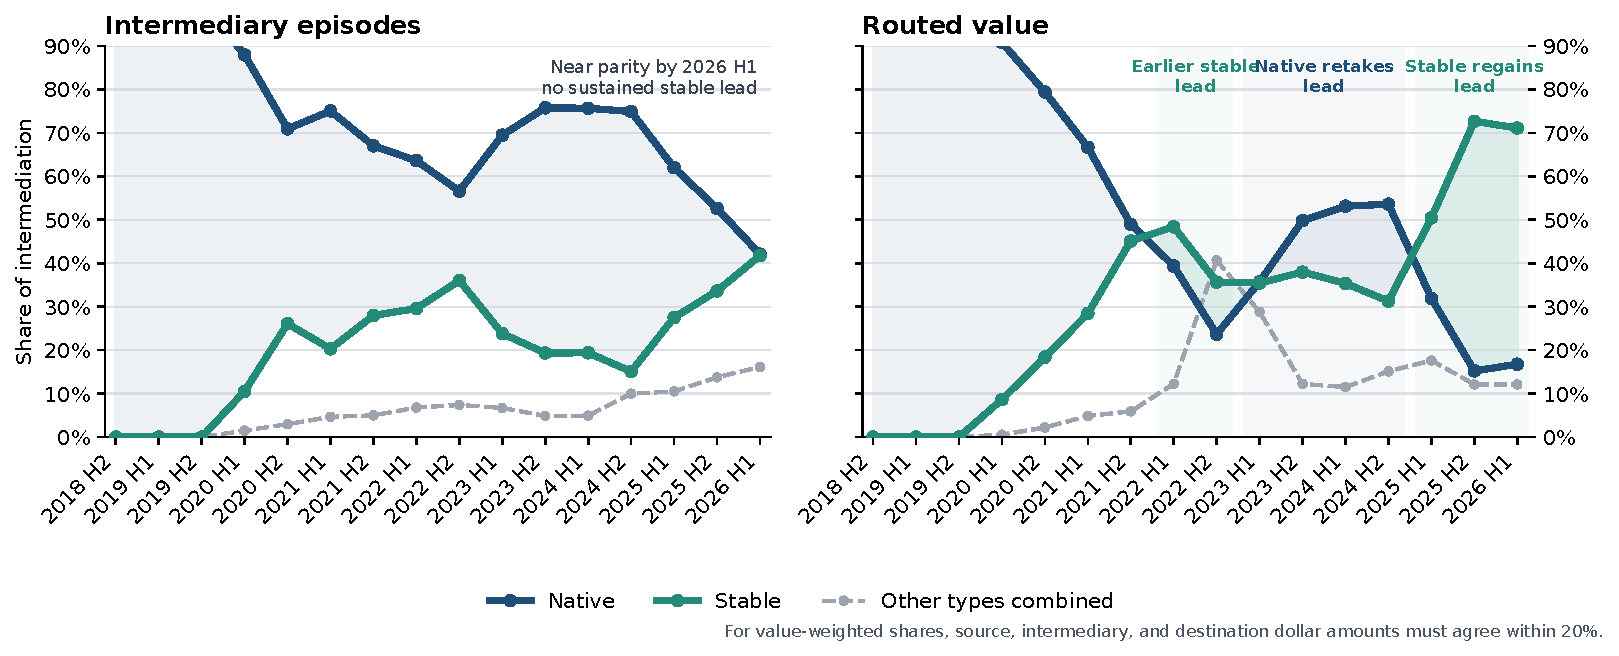
\includegraphics[width=0.98\textwidth]{../output/figures/experiments/annual_vehicle_composition_bands.pdf}
\exhibitnote{The sample contains complete routes that do not return to their starting asset. Each route contributes once for every intermediary it uses, so routes with more than two legs can contribute several observations. Shares are formed across all intermediary types; Appendix Table~\ref{tab:app:rotation} uses the narrower native-or-stable denominator. Every point covers six calendar months; the final point is 2026 H1. Routed value requires source, intermediary, and destination dollar amounts to agree within 20\%.}
\end{figure}

\subsection{Pair formation and persistence}
\label{sec:dominance:pairs}

Aggregate dominance can change inside continuing pairs or through the distribution of activity across pairs. Let $p$ denote a pair and $y\in\{2024,2026\}$. A continuing pair carries native-or-stable routes in both matched periods; a year-specific pair carries them in only one. First split total activity between these two sets. Within continuing pairs, stablecoin share can change because a given pair changes its vehicle mix or because trading shifts toward pairs with a different vehicle mix. The remaining change comes from the aggregate weight on continuing pairs and the stablecoin share of pairs observed in only one period.

Formally, let $W_y$ be the share of native-plus-stable activity in continuing pairs, $\omega_{p,y}$ pair $p$'s weight within that activity, and $s_{p,y}$ its stablecoin share. Continuing pairs have stablecoin share $S_{C,y}=\sum_p\omega_{p,y}s_{p,y}$, while year-specific pairs have share $S_{E,y}$. Total stablecoin share is therefore $S_y=W_yS_{C,y}+(1-W_y)S_{E,y}$. Writing $\Delta x=x_{2026}-x_{2024}$ and $\bar{x}=(x_{2024}+x_{2026})/2$ gives the exact midpoint decomposition
\begin{equation}
\label{eq:pair-decomposition}
\begin{aligned}
\Delta S={}&
\underbrace{\bar{W}\sum_p\bar{\omega}_p\Delta s_p}_{\text{switching within continuing pairs}}
+\underbrace{\bar{W}\sum_p\bar{s}_p\Delta\omega_p}_{\text{activity shifting across pairs}}\\
&+\underbrace{(\bar{S}_C-\bar{S}_E)\Delta W}_{\text{continuing-pair weight}}
+\underbrace{(1-\bar{W})\Delta S_E}_{\text{year-specific pairs}}.
\end{aligned}
\end{equation}

The midpoint averages hold the companion quantity fixed while each component changes, so the four terms add exactly to the aggregate change. The first two terms split the change among continuing pairs into changes in each pair's stablecoin share and changes in pair weights. The last two terms separate the changing mass of continuing pairs from the stablecoin share among period-specific pairs. The two sets partition each period's activity; nothing is deducted from a continuing pair.

We also compare the same pair, date within the year, and realised single- or cross-exchange route class. For route-count or routed-value stablecoin share $S^{(m)}_{pds,y}$, the matched regression is
\begin{equation}
\label{eq:pair-fe}
S^{(m)}_{pds,y}=\alpha^{(m)}_{pds}+\beta^{(m)}\mathbf{1}_{\{y=2026\}}+\varepsilon^{(m)}_{pds,y},
\qquad m\in\{N,V\}.
\end{equation}
Here $d$ is the month-day and $s$ the realised route class. Observations are weighted by native-plus-stable route count or supported routed value; standard errors cluster by pair and date. The comparison is descriptive because route class and trading activity can respond to the same forces as vehicle choice.

Table~\ref{tab:pair-composition} applies Equation~\eqref{eq:pair-decomposition} to route counts and supported value and reports Equation~\eqref{eq:pair-fe} on cells defined by pair, calendar date, and route class.

\FloatBarrier
\begin{table}[tbp]
\centering
\caption{Decomposition of the stablecoin rotation}
\label{tab:pair-composition}
\small
\begin{tabularx}{\linewidth}{@{}>{\raggedright\arraybackslash}Xrr@{}}
\toprule
Component or estimate & Estimate [pp] & Obs. \\
\midrule
\multicolumn{3}{l}{\emph{Panel A. Route-count share: continuing and year-specific pairs}} \\
Net stablecoin-share change within continuing pairs & $-0.1$ & \\
\quad Pairs moving toward stablecoins (1,569) & $+1.3$ & \\
\quad Pairs moving toward native assets (1,487) & $-1.4$ & \\
Vehicle activity shifting across continuing pairs & $+8.4$ & \\
Weight of continuing versus year-specific pairs & $-0.5$ & \\
Net contribution of period-specific vehicle activity & $+17.79$ & \\
\quad Pairs first observed after 2024 H1 & $+20.09$ & \\
\quad Pairs reactivated after absence in 2024 H1 & $+0.20$ & \\
\quad Vehicle-role turnover in continuing pairs & $-0.77$ & \\
\quad Pairs exiting before 2026 H1 & $-1.73$ & \\
\midrule
Total route-count change & $+25.5$ & \\
\addlinespace
\multicolumn{3}{l}{\emph{Panel B. Dollar-weighted share: continuing and year-specific pairs}} \\
Net stablecoin-share change within continuing pairs & $0.0$ & \\
\quad Pairs moving toward stablecoins (1,505) & $+2.3$ & \\
\quad Pairs moving toward native assets (1,445) & $-2.4$ & \\
Vehicle activity shifting across continuing pairs & $+26.2$ & \\
Weight of continuing versus year-specific pairs & $-2.5$ & \\
Net contribution of period-specific vehicle activity & $+19.16$ & \\
\quad Pairs first observed after 2024 H1 & $+21.94$ & \\
\quad Pairs reactivated after absence in 2024 H1 & $+0.04$ & \\
\quad Vehicle-role turnover in continuing pairs & $-1.72$ & \\
\quad Pairs exiting before 2026 H1 & $-1.10$ & \\
\midrule
Total change in dollar-weighted share & $+42.8$ & \\
\addlinespace
\multicolumn{3}{l}{\emph{Panel C. Matched pair estimates}} \\
\midrule
All two-leg routes, count share & $+0.23\ (0.77)$ & 188,344 \\
20\% agreement sample, count share & $+0.32\ (0.75)$ & 182,734 \\
20\% agreement sample, dollar-weighted share & $-1.35\ (2.19)$ & 182,734 \\
\bottomrule
\end{tabularx}

\exhibitnote{Panels A through C compare pooled activity over matched January--June dates in 2024 and 2026. Panels B and C report Equation~\eqref{eq:pair-decomposition}; their indented rows split the within-pair component into positive and negative contributions. Panel C weights routes by dollar value and applies the 20\% agreement rule. Panel D estimates Equation~\eqref{eq:pair-fe}; standard errors use two-way clustering by pair and date. Panels A and B factor the same route-count change in different ways, so their components should not be combined.}
\end{table}

Pooling route counts gives an increase from \PairPooledBase{} to \PairPooledEnd{}, or \PairPooledTotal{}, close to the equal-day change in Appendix Table~\ref{tab:app:rotation}. The within-pair component is \PairPooledWithin{} by route count and \PairValueWithin{} by routed value. These net estimates combine \MarginWithinGrossUp{} from pairs moving toward stablecoins and \MarginWithinGrossDown{} from pairs moving toward the native asset. Activity shifting across continuing pairs contributes \PairPooledReweight{} by count and \PairValueReweight{} by value. The changing aggregate weight on continuing pairs contributes \PairPooledSupportMass{} and \PairValueSupportMass{}, while year-specific pairs contribute \PairPooledExclusive{} and \PairValueExclusive{}. The last component is net of entry and exit: pairs observed only in 2026 add their later-period vehicle use, while pairs observed only in 2024 remove their earlier-period vehicle use. Equation~\eqref{eq:pair-fe} reaches the same conclusion on the more restrictive matched sample: stablecoin share changes by \MatchedMarketCountChange{} by count and \MatchedMarketValueChange{} by value. A large aggregate rotation therefore coexists with little net switching inside established cells defined by pair, calendar date, and route class.
% output/exhibits/vehicle_transition_pair_decomposition.jsonl; output/exhibits/vehicle_transition_pair_fixed_effects.jsonl

The same decomposition covers every adjacent January--June comparison between 2019 and 2026. As shown in Appendix Table~\ref{tab:app:rotation-boundaries}, panel A, the within-pair term ranges only from \AdjacentWithinMin{} to \AdjacentWithinMax{}, while aggregate changes range from \AdjacentLargestDecline{} in \AdjacentLargestDeclineYears{} to \AdjacentLargestIncrease{} in \AdjacentLargestIncreaseYears{}. Pair composition therefore accounts for both stablecoin gains and the intervening reversals.
% output/exhibits/vehicle_transition_adjacent_year_decomposition.jsonl; output/exhibits/result_resolution_values.tex

Endpoint demand clarifies the composition result. A pair with WETH at one endpoint cannot also use WETH as its intermediary, so part of the native-versus-stable allocation is mechanically fixed. Panel A of Appendix Table~\ref{tab:app:endpoint-direction} splits the headline daily change by endpoint direction. Pairs with one native and one stable endpoint contribute \EndpointNativeStableCountContribution{} by route count and \EndpointNativeStableValueContribution{} by routed value; pairs with two stable endpoints contribute \EndpointStableStableCountContribution{} and \EndpointStableStableValueContribution{}, respectively. All other pairs remain the largest channel overall. Panel B shows that USDT supplies \StableStableUsdtValueContribution{} of the two-stable-endpoint value increase, while USDC, DAI, and the remaining stablecoin intermediaries jointly contribute \StableStableOtherValueContribution{}. The result is present on all \StableStableActiveDays{} common days, and trimming the largest decile of daily contributions leaves a \StableStableTrimmedValueChange{} increase. Stablecoin dominance therefore spreads beyond pairs whose endpoint identity limits the native vehicle, while routing between stable currencies concentrates on one intermediary issuer.
% output/exhibits/vehicle_transition_pair_contributions.parquet; output/exhibits/vehicle_transition_pair_decomposition_deck_values.tex; output/exhibits/endpoint_direction_decomposition.jsonl; output/exhibits/endpoint_direction_deck_values.tex; output/exhibits/stable_stable_vehicle_decomposition.jsonl; output/exhibits/stable_stable_vehicle_robustness.jsonl; output/exhibits/stable_stable_vehicle_values.tex

Panel B of Appendix Table~\ref{tab:app:rotation-boundaries} removes every pair with WETH or a stablecoin at either endpoint. Stablecoin vehicle share still rises from \NonvehicleEndpointStableBase{} to \NonvehicleEndpointStableEnd{} by count and from \NonvehicleEndpointValueBase{} to \NonvehicleEndpointValueEnd{} by supported value. Pair entry and exit contribute \NonvehicleEndpointCountExclusive{} and \NonvehicleEndpointValueExclusive{}, respectively. The rotation therefore remains economically large among pairs for which both broad vehicle families are distinct from the assets being exchanged.
% output/exhibits/vehicle_transition_nonvehicle_endpoint_decomposition.jsonl; output/exhibits/result_resolution_values.tex

The first routes in a new pair predict its subsequent vehicle. For pair $p$, let $E_p$ be the stablecoin share on its entry day. For each of the disjoint windows $h\in\{1\text{--}30,31\text{--}120\}$, let $R_{p,h}$ indicate that the pair carries another native- or stablecoin-intermediated route, and let $S_{p,h}$ be the stablecoin share when $R_{p,h}=1$. We estimate
\begin{equation}
\label{eq:entry-persistence}
\begin{aligned}
S_{p,h}&=\alpha_h+\beta_h E_p+X_p'\delta_h+\varepsilon_{p,h},
&& R_{p,h}=1,\\
R_{p,h}&=a_h+b_h E_p+X_p'c_h+u_{p,h},
&& \text{all entrant pairs}.
\end{aligned}
\end{equation}
The second line is a linear probability model. The controls $X_p$ contain the cohort year, a stablecoin-endpoint indicator, log entry-day route count, direct-route share, and complex-route share. The sample uses pairs entering by March 2 in 2024 or 2026, giving every pair 120 complete calendar days of follow-up. Pairs with a native asset at either endpoint are excluded.

\FloatBarrier
\begin{table}[tbp]
\centering
\caption{Vehicle persistence after pair entry}
\label{tab:entry-persistence}
{\tiny
\renewcommand{\arraystretch}{0.90}
\begin{tabularx}{\linewidth}{@{}>{\hsize=1.6\hsize\raggedright\arraybackslash}X*{6}{>{\hsize=.9\hsize\centering\arraybackslash}X}@{}}
\toprule
\multicolumn{7}{@{}l}{\textit{Panel A. Stablecoin route share among pairs that trade again [\%]}} \\
 & \multicolumn{3}{c}{Days 1--30} & \multicolumn{3}{c}{Days 31--120} \\
\cmidrule(lr){2-4}\cmidrule(l){5-7}
 & (1) & (2) & (3) & (4) & (5) & (6) \\
\midrule
Entry stablecoin share [10 pp] & \begin{tabular}{@{}c@{}}$+9.00^{***}$\\$(0.14)$\end{tabular} & \begin{tabular}{@{}c@{}}$+8.92^{***}$\\$(0.15)$\end{tabular} & \begin{tabular}{@{}c@{}}$+8.55^{***}$\\$(0.72)$\end{tabular} & \begin{tabular}{@{}c@{}}$+8.59^{***}$\\$(0.18)$\end{tabular} & \begin{tabular}{@{}c@{}}$+8.40^{***}$\\$(0.18)$\end{tabular} & \begin{tabular}{@{}c@{}}$+9.00^{***}$\\$(0.50)$\end{tabular} \\
\addlinespace
Controls & No & Yes & Yes & No & Yes & Yes \\
Route-activity weights & No & No & Yes & No & No & Yes \\
Observations (pairs) & 30,547 & 30,547 & 30,547 & 19,405 & 19,405 & 19,405 \\
Entry-date clusters & 123 & 123 & 123 & 123 & 123 & 123 \\
Mean stablecoin share [\%] & 2.70 & 2.70 & 4.78 & 3.83 & 3.83 & 7.18 \\
$R^2$ & 0.842 & 0.843 & 0.800 & 0.787 & 0.791 & 0.830 \\
\bottomrule
\end{tabularx}

\vspace{0.65em}

\begin{tabularx}{\linewidth}{@{}>{\hsize=1.8\hsize\raggedright\arraybackslash}X*{2}{>{\hsize=.6\hsize\centering\arraybackslash}X}@{}}
\toprule
\multicolumn{3}{@{}l}{\textit{Panel B. Subsequent-trading incidence among all entrants [\%]}} \\
 & Days 1--30 & Days 31--120 \\
\midrule
Entry stablecoin share [10 pp] & \begin{tabular}{@{}c@{}}$+0.30^{***}$\\$(0.08)$\end{tabular} & \begin{tabular}{@{}c@{}}$+0.98^{***}$\\$(0.08)$\end{tabular} \\
Controls & Yes & Yes \\
Observations (pairs) & 157,262 & 157,262 \\
Entry-date clusters & 123 & 123 \\
Mean retrading rate [\%] & 19.42 & 12.34 \\
$R^2$ & 0.068 & 0.033 \\
\bottomrule
\end{tabularx}

}
\exhibitnote{Panel A estimates the first line of Equation~\eqref{eq:entry-persistence} among pairs that carry another native- or stablecoin-intermediated route in the stated window. Panel B estimates the second line on all entrant pairs. The entry day is excluded from both follow-up windows. Controls are the cohort year, a stablecoin-endpoint indicator, log entry-day route count, direct-route share, and complex-route share. Columns 3 and 6 weight pairs by route activity in the respective follow-up window; all other columns give each pair equal weight. Coefficients report the outcome change in percentage points (pp) associated with a 10 pp higher entry-day stablecoin share. Standard errors in parentheses use CR1 clustering by entry date. Asterisks \(*\), \(**\), and \(***\) denote statistical significance at the 10\%, 5\%, and 1\% levels, respectively.}
\end{table}

We separate later vehicle use from pair survival. Of the \EntryPersistenceEntrants{} entrants, \EntryPersistenceEarlyRetradeRate{} trade again during days 1--30 and \EntryPersistenceLateRetradeRate{} do so during days 31--120. Among pairs that trade again, a 10 pp higher entry-day stablecoin share predicts \EntryPersistenceEarlyPairEffectPerTen{} higher stablecoin share during days 1--30 and \EntryPersistenceLatePairEffectPerTen{} during days 31--120 (Table~\ref{tab:entry-persistence}, panel A, columns 2 and 5). The route-activity-weighted estimates are \EntryPersistenceEarlyActivityEffectPerTen{} and \EntryPersistenceLateActivityEffectPerTen{}, respectively (columns 3 and 6). Every follow-up outcome begins after the entry day, so these estimates capture continued vehicle use across subsequent routes.

The share estimates describe pairs that remain active in each window. Entry-day stablecoin share also predicts a modestly higher probability of subsequent trading: a 10 pp increase corresponds to \EntryPersistenceEarlyRetradeEffectPerTen{} during days 1--30 and \EntryPersistenceLateRetradeEffectPerTen{} during days 31--120 (Table~\ref{tab:entry-persistence}, panel B). The evidence therefore combines strong persistence in vehicle identity among surviving pairs with a smaller survival margin. We interpret both as descriptive equilibrium relationships: relative prices, depth, and venue access can shape the vehicle at entry and remain relevant for later trading.
% output/exhibits/entry_vehicle_persistence_models.jsonl; output/exhibits/entry_vehicle_persistence_support.jsonl; output/tables/entry_vehicle_persistence.tex

Network reach, issuer-level specialisation, within-day endpoint demand, and exchange span provide supplementary views of the same formation result. Appendix~\ref{app:additional-composition} reports these estimates. They show that stablecoin arrival is more common in older and more active pairs, intermediary use moves closely with a currency's endpoint demand within a day, and the stablecoin rotation appears in both single- and cross-exchange routes. These comparisons help locate the result but do not replace the direct decomposition in Table~\ref{tab:pair-composition}.

% Counterfactual prices are discussed only to bound the route evidence.

\section{A counterfactual execution-cost benchmark}
\label{sec:executability}

Realised routes identify the assets that carried each trade. Relating that choice to execution costs requires the alternatives available immediately beforehand, quoted at the same trade size and over the exchanges the trader or router could reach. The route-composition results use observed paths directly; the cost comparison adds this counterfactual set.

We hold the source, destination, input amount, and pre-transaction pool state fixed, then compare the output of the best direct path with the best two-leg path through a specified intermediary. This extends the realised-versus-optimised benchmark for allocations among parallel pools \citep{XiMoallemi2026Routing} to sequential routes. Swaps and liquidity changes are replayed in their on-chain order because a daily or hourly closing state may contain information that arrived after the route was chosen. Hypothetical trades must also remain within a 5\% own-price-impact limit in every pool. Appendices~\ref{app:state} and~\ref{app:support} give the state reconstruction, pricing equations, and validation exercises.
% output/exhibits/quoter_support_bounds.jsonl; common 5 percent target support rule

The comparison is defined over public on-chain liquidity. A router may search a narrower set, and private order flow, financing costs, or losses from reverted transactions may affect its decision. Historical state also differs in quality across pool designs. In a sampled Curve exercise, pools that cannot be represented by the StableSwap model account for 34.2\% of assessed volume and are concentrated in native-asset markets: 65.2\% of native-leg volume, compared with 21.1\% of stablecoin-leg volume. Hook-bearing or dynamic-fee Uniswap v4 pools, SushiSwap v3 pools without historical state, and several Balancer families require separate pricing models. Appendix~\ref{app:coverage} reports these coverage comparisons.
% docs/venue-coverage-bounds.md; output/exhibits/curve_excluded_composition.jsonl

\section{What can account for the rotation?}
\label{sec:rivals}

The allocation results sharpen the mechanism question. Stablecoin dominance rose chiefly as routed activity moved across source--destination pairs and the incidence of intermediation changed, while repeated replacement of a native intermediary within continuing pairs contributed little. Any explanation for the rotation must therefore account for the assets being exchanged as well as the intermediary carrying the route.

\subsection{Path complexity and exchange span}
\label{sec:rivals:complexity}

Does the rotation follow from how routes are assembled rather than from which asset intermediates them? Paths grew longer and reached across more exchanges over the sample, and long paths already favoured stablecoins: in 2024 stablecoins carried \MultiLegCountBase{} of native-plus-stable intermediary episodes on routes of more than two legs, against \StableCountBase{} on two-leg routes. An account in which construction does the work therefore predicts a specific pattern. The stablecoin share should be roughly flat inside a complexity class, and the aggregate increase should come from the movement of activity toward the longer routes that were already stablecoin-intensive.

Neither part holds. Among intermediary episodes on two-leg routes, the stablecoin share rises \StableCountChange{} by count, with a standard error of \StableCountSE{}, and \StableValueChange{} by value (\StableValueSE{}). Among episodes on routes of more than two legs it rises \MultiLegCountChange{} (\MultiLegCountSE{}) and \MultiLegValueChange{} (\MultiLegValueSE{}), from a base of \MultiLegCountBase{} to \MultiLegCountEnd{} by count. Both classes move, and the class with the shortest paths moves further, so reweighting toward complex routes cannot supply the aggregate change. Dividing each complexity class again by whether the route touched one exchange or several leaves four groups, and every one of them rises; the weakest is \WeakestComplexityCountChange{} by count (\WeakestComplexityCountSE{}) and \WeakestComplexityValueChange{} by value (\WeakestComplexityValueSE{}). The stablecoin gain is thus common to short and long paths and to routes that stay on one exchange and routes that do not.

Two boundaries limit what this comparison licenses. The number of legs records the path a trade actually took, so it measures how the route was built and not how well it was chosen; a route with more legs is not thereby a worse or a better execution. Complexity and exchange span are also outcomes rather than assignments, since the same conditions that make a longer or wider path attractive can bear on the choice of intermediary. The comparison rules out a composition account of the rotation; it does not identify an effect of routing software or of the exchange set on which asset intermediates a trade.
% output/exhibits/intermediation_complexity_rival.jsonl (evidence commit 111230a) via
% output/exhibits/provisional_results_deck_values.tex (macros; producer
% src/ddvc/provisional_results.py). Route-only certified evidence: matched
% January--June dates in 2024 and 2026, native-plus-stable denominator, one
% observation per intermediary episode, 30-day Newey--West standard errors.
% The four scope-by-complexity cells are rendered through a producer that
% refuses to emit the joint statement unless all four changes are positive.

\subsection{Liquidity in the vehicle's own pools}
\label{sec:rivals:capital}

The classical vehicle-currency mechanism links trading volume to lower transaction costs \citep{Krugman1980VehicleCurrencies}. On a decentralised exchange, the relevant markets are the pools connecting an intermediary to other assets. Trading can attract provider capital, deeper pools can lower price impact, and lower price impact can draw further trading. Pool size remains an equilibrium outcome because providers balance fee income against adverse-selection risk and the cost of adjusting their positions \citep{LeharParlour2024Uniswap}. Deposited capital measures funds committed to a pool; a size-specific quote measures how much liquidity is executable within a stated price impact. The distinction matters. Concentrated-liquidity providers can alter executable depth by changing where capital is placed along the price curve, so deposited capital and executable liquidity coincide only under particular pool designs \citep{AdamsZinsmeisterRobinson2021UniswapV3}.

That mechanism operates inside a market. Deeper pools joining stablecoins to other assets reduce the price impact of carrying a given source--destination trade through a stablecoin, so the classical account asks the trader to switch intermediary in a pair that was already being traded. Section~\ref{sec:dominance:pairs} measures exactly that margin, and it is the one that stays still: within pairs traded in both years, the stablecoin share changes by \MatchedMarketCountChange{} by count, and the interval around it excludes within-pair increases beyond \MatchedMarketCountCIUpper{}. Depth in stablecoin pools cannot therefore carry the rotation through continuing markets. What it can still do is act earlier, by making a stablecoin the asset to which a newly traded or fast-growing pair is connected when its markets are first formed. Separating the two roles calls for the capital committed to each candidate's pools on the same daily calendar as the routes, read in each direction on its own, because a contemporaneous association between trading and depth is equally consistent with either.
% The reciprocal V2 deposited-capital and vehicle-use estimates exist but are
% not reproducible at this evidence generation: the runner fails closed without
% its D3 binding (see logs/grind-ledger.md, 2026-08-16). No coefficient from
% that estimator enters the manuscript until it reruns and reproduces.

\subsection{Protocol architecture}

Protocol design changes the set of routes that can be formed. Uniswap v1 created pools between an ERC-20 token and ETH, so token-to-token trades crossed ETH; Uniswap v2 allowed arbitrary ERC-20--ERC-20 pools and made direct token-to-token trading possible.\footnote{See Adams, Zinsmeister, and Robinson, \href{https://docs.uniswap.org/whitepaper.pdf}{\emph{Uniswap v2 Core}}, pp.~1--2.} Forced intermediation was material while the constraint lasted: token-to-token trades routed through ETH account for 8.0\% of Uniswap v1 swap transactions and 8.1\% of its ETH volume over the venue's life, and roughly one trade in ten in 2019 and 2020, when the venue was most active. A transaction from the crash weekend of March 2020 shows the mandate operating: with no direct pool between MKR and DAI, a trader selling \VOneCaseTokenIn{} MKR received \VOneCaseEth{} ETH at one exchange contract and spent the identical ETH amount at a second for \VOneCaseTokenOut{} DAI.\footnote{Transaction \ethtx{\VOneCaseTx}{\VOneCaseTxShort}, block \VOneCaseBlock, March 15, 2020. The trace is selected by a deterministic rule, the largest ETH amount routed among the \VOneCaseExactCount{} mandate-era token-to-token transactions whose two ETH legs match exactly, and the token identities are verified against the public transfer record.} Native-asset pairing remained pervasive after this mandate ended. The share of single-leg Uniswap v2 trades executed in WETH pools was 95.1\% in 2020 and 95.5\% in 2026, remaining between 93.4\% and 97.9\% in every intervening year. Among the 477,633 pairs that ever traded on Uniswap v2, 97.1\% include WETH, and WETH's share of newly traded pairs rose from 84.1\% in 2020 to 97.9\% in 2026. This persistence is consistent with deep WETH pools, launch conventions, and inherited search paths. Separating those forces from the original protocol constraint requires comparison among pairs that had the same alternatives available.
% docs/finding-v1-forced-vehicle.md; output/exhibits/v1_forced_vehicle_report.md
% Registered case: output/exhibits/v1_route_case.json via output/exhibits/v1_route_case_deck_values.tex
% (macros; producer scripts/build_v1_route_case.py, evidence commit 38aaa86). Composition shares
% 7.97% of swaps / 8.11% of ETH volume (whole sample) and the 2019--2020 ~10% monthly shares are the
% docs/finding-v1-forced-vehicle.md section 1 composition table and monthly t2t_share series.

Uniswap v4 separates route choice from physical settlement more sharply. All pools reside in one singleton, and flash accounting records balance changes internally before settling the final net amounts at the end of a call.\footnote{See Adams et al., \href{https://app.uniswap.org/whitepaper-v4.pdf}{\emph{Uniswap v4 Core}}, Sections 1 and 3.} An economic route can therefore cross an intermediary pool without generating an external token transfer at every step. Decoded pool actions preserve the trading path despite this netting, while the architecture changes how liquidity, fees, and settlement are organised around that path.

The route evidence leaves an explanation three features to account for. The stablecoin gain occurs mainly across pairs rather than through repeated substitution within matched pairs; it appears on short and long paths alike and on routes that stay within one exchange as well as routes that do not; and the measured WETH-pairing persistence shows that route opportunities can outlast the protocol rule that first created them. Together these narrow the candidates. An explanation cannot rest on the composition of the routes that were built, and it cannot rest on repeated intermediary substitution in established markets. It has to say why the markets forming and growing over this period attach themselves to a stablecoin.

% Conclusion restricted to the current route-only findings registry.

\section{Conclusion}
\label{sec:conclusion}

Realised trading paths make vehicle-currency use directly observable. They separate the assets that ever intermediate a trade from the smaller set that carries most routed activity. In our sample, stablecoins become the leading vehicles by value relative to native assets, although the transition reverses more than once. USDT accounts for most of the increase within the stablecoin category.

Where trading occurs is central to this transition. Most of the increase comes from endpoint pairs entering or leaving, changes in activity among continuing pairs, and greater use of indirect routes. Direct stable-for-native switching inside continuing markets contributes little. A model that holds the set of markets fixed therefore captures only part of the formation of vehicle dominance.

The usual liquidity feedback begins with currency choice inside an established market: greater use deepens liquidity and makes future use more attractive. The route evidence adds a market-formation margin. Changes in which pairs trade and which of them route indirectly can extend the pools and software support associated with a currency even when intermediary choice inside a continuing market changes little.

Liquidity provision, venue reach, endpoint demand, and routing software may explain why activity moved toward USDT-centred routes; realised paths alone cannot separate these mechanisms. What the paths establish is that vehicle dominance is shaped by the formation of routed markets as well as by the choice of intermediary within markets already in place.

\clearpage
% Appendix. The construction and validation apparatus behind the constructed side of every
% cost comparison in the body.
%
% Same provenance discipline as the body sections: every numeric prose line and every
% tabular row carries a trailing comment naming the artefact it was read from and the
% sample it was measured on. A row is where a reader checks a number, so the comment sits
% on the row and not only on the table.

\appendix

\section{From contract events to economic routes}
\label{app:route-construction}

Each exchange records trades in its own contract and event format. We first identify pools from the protocol's factory or registry, map contract addresses to tokens, and convert raw integer amounts using the token precision that applied at the time of the trade. Contract addresses define token identity because unrelated tokens can share a symbol and the same economic asset can appear in native and wrapped form. We consolidate ETH and WETH only after the address-level reconstruction; every other token remains distinct unless a stated economic classification combines it.

We then order all swap events within a transaction by block, transaction, and log position. The ordered token flows reveal the exchange that actually occurred. A single connected chain gives one route, parallel chains identify an order split, and disconnected event groups remain separate. This procedure is necessary because one transaction can contain unrelated calls as well as trades across several exchanges. It also prevents a transaction with two simultaneous routes from being mistaken for one longer route. The output is the sequence of assets and pools traversed, not an inference from the transaction sender or router label.

The route-count sample requires a complete token sequence but not a dollar price. The value-weighted sample additionally requires every leg to have coherent amounts and a common dollar valuation. Failed valuation therefore removes an observation from the value calculation without erasing the observed route. Self-returning paths are excluded under the rule in Appendix~\ref{app:roundtrip}, since they do not exchange one endpoint asset for another.

Historical token precision cannot be verified for 13 tokens traded in 22 constant-product pools. Reserve-reconstruction analyses omit those pools. A deliberately conservative check removes every route involving any of the 13 tokens: the resulting upper bound is 5,950 routes and \$10.91 million of route value. Only 1,036 of those routes use one of the affected tokens as an intermediary, representing \$1.284 million, or 0.00043\% of value on routes whose legs can all be valued. All 13 tokens lie outside the native and stablecoin groups used in the main comparison. The exclusion affects exact reserve reconstruction; the route-composition result is unchanged.
% docs/findings-freeze.md, 13 unresolved V2 token-precision records and worst-case route deletion bound

This separation follows the treatment of blockchain data in \citet{LeharParlour2024Uniswap} and \citet{GriffinShams2020Untethered}, and the broader practice of reporting identity rules and unmatched observations in \citet{BoltonKacperczyk2021CarbonRisk}. The main analysis states the economic sample and measurement; the appendix reports event ordering, exclusions, and their quantitative importance.

\section{Quoter construction and validation}
\label{app:quoters}

The constructed side of every comparison in the body is an exact-input quote: given a pool's state and an input amount, what would the pool have paid out? Each venue family is priced with its own invariant and arithmetic. We assess each implementation by reconstructing the state immediately before executed swaps and comparing predicted with realised output. Curve's amplification coefficient and Balancer's weight ratio are not available in the historical subgraph records, so we estimate them from realised trades and evaluate the resulting quotes on separate trades.

\subsection{Constant-product pools}
\label{app:quoters:cp}

Uniswap v2 and SushiSwap v2 price the product of reserves \citep{LeharParlour2024Uniswap}. With input reserve $R_{\mathrm{in}}$, output reserve $R_{\mathrm{out}}$, input amount $x$ and the fee factor $\phi$, an exact-input swap moves the pool along
\[
(R_{\mathrm{in}} + \phi x)\,(R_{\mathrm{out}} - y) \;=\; R_{\mathrm{in}} R_{\mathrm{out}},
\]
which inverts in closed form to
\[
y(x) \;=\; \frac{\phi\, x\, R_{\mathrm{out}}}{R_{\mathrm{in}} + \phi\, x}, \qquad \phi = \tfrac{997}{1000},
\]
the 30 basis point fee both venues charge, applied on chain as the integer ratio above.
% src/ddvc/cpquote.py, FEE_NUM and FEE_DEN, Uniswap v2 and SushiSwap v2

A multi-leg route composes these one hop at a time, threading the output token of one pool into the next, and the route-cost gap the body reports is the basis-point margin by which the best direct quote beats the best intermediated quote at the same state and the same size,
\[
g \;=\; 10^{4}\,\frac{q_{\mathrm{direct}} - q_{\mathrm{via}}}{q_{\mathrm{via}}}.
\]
Both sides of $g$ are computed from one reconstructed state, which is the property the realised-trade comparison lacked and the reason the counterfactual exists at all.

Quoting each executed swap against the state immediately before it gives a median absolute error of 0.0000\% across 8,024 swaps; 96.7\% of quotes are within 1\% and 95.2\% are within 0.01\% of realised output.
% src/ddvc/cpquote.py module docstring, 8,024 executed swaps

\subsection{Concentrated liquidity}
\label{app:quoters:cl}

Uniswap v3 and v4 distribute reserves across price ranges, so a pool has no single reserve pair and a quote has to walk the price axis \citep{AdamsZinsmeisterRobinson2021UniswapV3}. Inside one range the pool behaves as a constant-product pool with virtual reserves, and liquidity $L$ with price $P$ satisfies
\[
L = \sqrt{x\,y}, \qquad \sqrt{P} = \sqrt{y/x},
\]
so the amounts consumed and paid out over a price move from $\sqrt{P_a}$ to $\sqrt{P_b}$ are
\[
\Delta x = L\left(\frac{1}{\sqrt{P_a}} - \frac{1}{\sqrt{P_b}}\right), \qquad \Delta y = L\left(\sqrt{P_b} - \sqrt{P_a}\right).
\]
An exact-input step inverts those. Paying in token1 raises the price by a linear increment in root price, and paying in token0 lowers it through a reciprocal update,
\[
\sqrt{P'} = \sqrt{P} + \frac{\Delta y}{L}, \qquad \sqrt{P'} = \frac{L\sqrt{P}}{L + \Delta x \sqrt{P}}.
\]
Range boundaries sit on a geometric tick grid and each initialised tick carries a signed liquidity delta applied on crossing,
\[
\sqrt{P(i)} = 1.0001^{\,i/2}, \qquad L \mapsto L \pm \Delta L_i ,
\]
with the sign set by the direction of travel. The quoter carries the contract's own integer Q96 arithmetic, including the round-up conventions on the input side and the round-down conventions on the output side, so a quote is exact given the state.
% src/ddvc/pricing/v3quote.py, integer port of SwapMath.computeSwapStep and TickMath

The active tick map is accumulated from every mint and burn strictly before the validation day, then same-day liquidity changes and swaps are replayed together by block and log index. Consecutive swaps in one pool supply the price state: the earlier event leaves \texttt{sqrtPriceX96} and \texttt{tick} immediately before the later swap, while the interleaved event stream supplies the active liquidity it actually faced. Errors are reported by trade direction crossed with whether the quote traversed an initialised tick, because a traversal fault is directional by construction and a pooled error statistic averages a broken direction against a working one. This failure occurred in validation: an upward search that returned the tick just crossed produced a zero-width step and under-quoted upward tick-crossing swaps by a median 62.6\%, while every non-crossing quote read exact and the downward direction validated at $-0.0006\%$.
% src/ddvc/pricing/v3quote.py, _next_init_tick measured docstring against realised swaps

Table~\ref{tab:app:cl} reports four validation groups on Uniswap v4, whose supported pools exercise the same code path on static fee tiers v3 never carried, including 0, 7, 8 and 20,000 hundredths of a basis point. Hook-bearing and dynamic-fee pools are excluded because their transaction-level cash flows and realised fee are not present in the raw records; Appendix~\ref{app:coverage} reports their share of v4 trading.
% output/exhibits/v4_quoter_validation.jsonl, observed static fee tiers; output/exhibits/v4_quote_support.jsonl, support statuses

\begin{table}[t]
\centering
\caption{Concentrated-liquidity quoter, by direction and tick crossing}
\label{tab:app:cl}
\begin{tabular}{lrrrrr}
\toprule
Validation group & Swaps & Median & 90th pct. & Maximum & Within 1\% \\
% output/exhibits/v4_quoter_validation.jsonl, column headings for 4,218 validated v4 swaps
\midrule
token0 in, no tick crossed & 2{,}290 & $0$ & $0$ & $9.98\times10^{-4}$ & 100.0\% \\
% output/exhibits/v4_quoter_validation.jsonl, 2,290 of 4,218 validated v4 swaps
token0 in, tick crossed & 57 & $0$ & $0$ & $3.45\times10^{-7}$ & 100.0\% \\
% output/exhibits/v4_quoter_validation.jsonl, 57 of 4,218 validated v4 swaps
token1 in, no tick crossed & 1{,}816 & $0$ & $1.69\times10^{-8}$ & $1.48\times10^{-4}$ & 100.0\% \\
% output/exhibits/v4_quoter_validation.jsonl, 1,816 of 4,218 validated v4 swaps
token1 in, tick crossed & 55 & $0$ & $5.44\times10^{-9}$ & $8.74\times10^{-9}$ & 100.0\% \\
% output/exhibits/v4_quoter_validation.jsonl, 55 of 4,218 validated v4 swaps
\midrule
Pooled & 4{,}218 & $0$ & $1.15\times10^{-14}$ & $9.98\times10^{-4}$ & 100.0\% \\
% output/exhibits/v4_quoter_validation.jsonl, all 4,218 validated v4 swaps
\bottomrule
\end{tabular}
\\[4pt]
\footnotesize Absolute quote error in percent of realised output. 4,218 realised Uniswap v4 swaps on three dates across 13 pools and nine pairs, at static fee tiers 0, 7, 8, 100, 500, 10,000 and 20,000. Each quote uses liquidity events ordered strictly before the swap and the price state left by the preceding swap in the same pool.
\end{table}

The four validation groups sit at the same location because the split isolates direction and tick crossing. Every group reproduces realised output within 0.001\% at the worst observed swap, against route-cost differences the body measures in tens of basis points.
% output/exhibits/v4_quoter_validation.jsonl, maximum absolute error 0.000998 percent over 4,218 swaps

\subsection{StableSwap pools}
\label{app:quoters:stable}

Curve interpolates between a constant-sum curve, which is flat and charges no slippage, and the constant-product curve of Section~\ref{app:quoters:cp}. For $n$ tokens with balances $x_i$, amplification $A$ and invariant $D$,
\[
A n^{n} \sum_i x_i + D \;=\; A D n^{n} + \frac{D^{\,n+1}}{n^{n} \prod_i x_i},
\]
where $A \to 0$ recovers the constant product and $A \to \infty$ recovers the constant sum. The contract solves $D$ by Newton iteration and an exact-input quote solves the same equation for the output balance once the input balance is raised, so with $D_{p} = D \prod_k D / (n x_k)$ the two loops are
\[
D \;\leftarrow\; \frac{\left(A n \sum_i x_i + n D_p\right) D}{(A n - 1) D + (n+1) D_p}, \qquad y \;\leftarrow\; \frac{y^{2} + c}{2y + b - D},
\]
with $b$ and $c$ formed from the balances of the tokens the swap does not touch. Balances are rescaled to eighteen decimals before either loop runs, because the invariant treats its tokens as interchangeable at par and a six-decimal stablecoin read on an eighteen-decimal scale is off by a factor of $10^{12}$. Output is net of the pool fee,
\[
y_{\mathrm{net}} = (x_j - y - 1)\,(1 - f),
\]
carrying the contract's own off-by-one guard on the raw difference.
% src/ddvc/pricing/stableswap.py, get_d, get_y and quote_exact_input

$A$ is Curve-specific and the standardised subgraph schema drops it, so it is identified from data instead of fetched. Every other quantity in the invariant is observed and every Curve swap reports both amounts, which leaves $A$ as the only unknown,
\[
\widehat{A} \;=\; \arg\min_{A} \; Q_{0.90}\!\left\{ \frac{|q(A; x, f, \Delta_{\mathrm{in}}) - \Delta_{\mathrm{out}}|}{\Delta_{\mathrm{out}}} \right\},
\]
fitted on the first half of a pool-day's trades over a logarithmic grid with a ternary refinement, then evaluated on the trades not used for estimation. A pool-day is retained when the 90th percentile of fitting error is below 1\%. Using the upper tail prevents a partial fit from passing: one misspecified pool produced a median fitting error below 0.1\% but a 34\% median error on the other trades because the invariant fit only part of its activity.
% src/ddvc/pricing/stableswap.py, FIT_QUANTILE 0.90 and MAX_CALIBRATION_ERROR 0.01

Curve has also operated crypto-pools since 2021 that follow the CryptoSwap invariant. Applying StableSwap to these pools yields a best-fit $A$ of 3 and a 36\% median quote error. We therefore exclude pool-days whose observed trades are inconsistent with the StableSwap pricing rule.
% src/ddvc/pricing/stableswap.py, A_MIN comment recording the measured failure

\begin{table}[t]
\centering
\caption{StableSwap calibration and held-out quote error, by validation day}
\label{tab:app:curve}
\small
\begin{tabular}{lrrrrrr}
\toprule
Day & Pools fitted & Pools excluded & Held-out trades & Median $\widehat{A}$ & Median error & Within 1\% \\
% output/exhibits/curve_quoter_validation.jsonl, column headings for four sampled Curve days
\midrule
2021-05-28 & 9 & 14 & 367 & 12{,}716 & 0.030\% & 100.0\% \\
% output/exhibits/curve_quoter_validation.jsonl, 367 held-out Curve trades on 2021-05-28
2022-09-12 & 11 & 16 & 262 & 20{,}493 & 0.029\% & 100.0\% \\
% output/exhibits/curve_quoter_validation.jsonl, 262 held-out Curve trades on 2022-09-12
2023-12-28 & 20 & 28 & 471 & 23{,}428 & 0.039\% & 98.9\% \\
% output/exhibits/curve_quoter_validation.jsonl, 471 held-out Curve trades on 2023-12-28
2025-04-13 & 42 & 50 & 1{,}207 & 46{,}851 & 0.036\% & 99.7\% \\
% output/exhibits/curve_quoter_validation.jsonl, 1,207 held-out Curve trades on 2025-04-13
\bottomrule
\end{tabular}
\\[4pt]
\footnotesize four sampled days. $\widehat{A}$ is reported in the module's convention, which carries the on-chain precision factor of 100. Median error is the median absolute deviation of the quote from realised output on trades the calibration never saw.
\end{table}

Across four validation days, held-out median errors range from 0.029\% to 0.039\%. The fitted amplification coefficient rises over the sample as the composition of retained Curve pools shifts toward tighter stablecoin baskets.
% output/exhibits/curve_quoter_validation.jsonl, four sampled days from 2021-05-28 to 2025-04-13

\subsection{Weighted pools}
\label{app:quoters:weighted}

Balancer weighted pools keep a weighted geometric mean constant,
\[
\prod_i B_i^{\,W_i} = \mathrm{const}, \qquad \sum_i W_i = 1,
\]
which gives the two-token exact-input form
\[
y_{\mathrm{out}} \;=\; B_{\mathrm{out}}\left[\,1 - \left(\frac{B_{\mathrm{in}}}{B_{\mathrm{in}} + \phi\, x_{\mathrm{in}}}\right)^{W_{\mathrm{in}}/W_{\mathrm{out}}}\right].
\]
Only the ratio $W_{\mathrm{in}}/W_{\mathrm{out}}$ enters, so an equal-weight Balancer pool and a constant-product pair with the same balances quote identically and every departure is the weight ratio doing work. Quotes are refused past the vault's cap of 30\% of the input token's balance, because a swap beyond that reverts on chain and a number returned there would be a price the panel could not have traded.
% src/ddvc/pricing/weighted.py, MAX_IN_RATIO at 30% of the input balance

The weight ratio and the swap fee are both reported by the subgraph and both can be stale, since the schema serves them at the head block while balances come from a historical snapshot. Liquidity-bootstrapping pools move weights on a schedule and any weighted pool's owner can reset the fee, and the fee case showed up in validation before it was diagnosed: read parameters reproduced 2024 trades to $10^{-9}$ percent and 2022 trades only to 0.19\%, a fee-sized gap, since the fee enters through $\phi$ and a fee wrong by a basis point moves a quote by about a basis point. Both parameters are therefore identified the way Curve's $A$ is, with reading tried first and each fit introducing exactly one free scalar over at least four observations on the pair.
% src/ddvc/pricing/weighted.py, parameter identification docstring and MIN_PAIR_OBSERVATIONS

We retain a Balancer pool-day when the 90th percentile fitting error is below 0.1\%. The threshold separates weighted pools, whose held-out errors range from $10^{-9}$ to 0.004\%, from stable, composable-stable, and elliptic-curve pools, whose held-out errors range from 0.05\% to 1.08\% and have a 99th percentile of 12\%.
% src/ddvc/pricing/weighted.py, MAX_CALIBRATION_ERROR at 0.001 with the measured separation

\begin{table}[t]
\centering
\caption{Weighted-pool quoter, and what the snapshot instant is worth}
\label{tab:app:weighted}
\begin{tabular}{lrrrrr}
\toprule
Day & Held-out trades & Backward & Flat & Opening & Pools priced / excluded \\
\midrule
2021-04-25 & 4 & $4.7\times10^{-9}$ & 3.00\% & 3.94\% & 1 / 0 \\
% output/exhibits/weighted_quoter_validation.jsonl, 4 held-out Balancer trades on 2021-04-25
2021-09-29 & 273 & $2.5\times10^{-8}$ & 1.24\% & 0.80\% & 18 / 8 \\
% output/exhibits/weighted_quoter_validation.jsonl, 273 held-out Balancer trades on 2021-09-29
2022-03-09 & 524 & $1.6\times10^{-4}$ & 1.05\% & 2.66\% & 25 / 4 \\
% output/exhibits/weighted_quoter_validation.jsonl, 524 held-out Balancer trades on 2022-03-09
2022-08-16 & 701 & $1.1\times10^{-9}$ & 0.75\% & 1.04\% & 33 / 12 \\
% output/exhibits/weighted_quoter_validation.jsonl, 701 held-out Balancer trades on 2022-08-16
2023-01-24 & 832 & $2.0\times10^{-10}$ & 3.73\% & 4.71\% & 44 / 11 \\
% output/exhibits/weighted_quoter_validation.jsonl, 832 held-out Balancer trades on 2023-01-24
2023-07-03 & 301 & $7.1\times10^{-10}$ & 1.78\% & 3.32\% & 26 / 19 \\
% output/exhibits/weighted_quoter_validation.jsonl, 301 held-out Balancer trades on 2023-07-03
2023-12-11 & 185 & $2.8\times10^{-9}$ & 1.77\% & 2.91\% & 17 / 20 \\
% output/exhibits/weighted_quoter_validation.jsonl, 185 held-out Balancer trades on 2023-12-11
2024-05-20 & 265 & $3.8\times10^{-10}$ & 4.81\% & 5.17\% & 15 / 36 \\
% output/exhibits/weighted_quoter_validation.jsonl, 265 held-out Balancer trades on 2024-05-20
2024-10-27 & 142 & $1.8\times10^{-10}$ & 1.68\% & 2.24\% & 12 / 36 \\
% output/exhibits/weighted_quoter_validation.jsonl, 142 held-out Balancer trades on 2024-10-27
2025-04-06 & 248 & $2.1\times10^{-10}$ & 5.32\% & 9.48\% & 19 / 40 \\
% output/exhibits/weighted_quoter_validation.jsonl, 248 held-out Balancer trades on 2025-04-06
2025-09-13 & 501 & $2.5\times10^{-4}$ & 1.09\% & 1.71\% & 27 / 25 \\
% output/exhibits/weighted_quoter_validation.jsonl, 501 held-out Balancer trades on 2025-09-13
2026-02-21 & 582 & $8.7\times10^{-9}$ & 0.68\% & 1.90\% & 19 / 6 \\
% output/exhibits/weighted_quoter_validation.jsonl, 582 held-out Balancer trades on 2026-02-21
\bottomrule
\end{tabular}
\\[4pt]
\footnotesize Median absolute quote error in percent of realised output, on trades no fit ever saw. \emph{Backward} reconstructs per-swap balances by rolling the day's event sequence back from the closing snapshot, \emph{Flat} keeps the snapshot balances constant across the day, and \emph{Opening} treats the snapshot as the day's opening state and rolls forward. The sample contains twelve days from 2021-04 to 2026-02.
\end{table}

Across the twelve days, backward reconstruction returns a median error of 0.0000\% and identifies 256 of 473 testable pool-days as weighted pools. The excluded pool-days carry a median 91.8\% of tested swap volume, which materially limits the venue coverage of the counterfactual comparison.
% output/exhibits/weighted_quoter_validation.jsonl, 12 days, 256 priced and 217 excluded pool-days

\section{Reconstructing pool balances before each trade}
\label{app:state}

Every counterfactual quote needs the pool state immediately before the trade. The historical records instead store balances at the end of an hour or day. We recover the earlier state by ordering every balance-changing event within the period and unwinding the sequence from the recorded closing balance.

Let $R^{\mathrm{end}}$ be the stored period-end reserve pair and $\Delta_t$ the net signed amounts of the $t$-th event in execution order. The state before event $s$ is the stored value with every later event removed,
\[
R^{\mathrm{pre}}_{s} \;=\; R^{\mathrm{end}} - \sum_{t \ge s} \Delta_t \;=\; R^{\mathrm{pre}}_{s+1} - \Delta_s ,
\]
which is a single reverse pass over the period. The alternative reading takes the previous period's stored value as the current period's opening state and replays forward,
\[
\widetilde{R}^{\,\mathrm{pre}}_{s} \;=\; R^{\mathrm{end}}_{\mathrm{prev}} + \sum_{t < s} \Delta_t ,
\]
which accumulates every unrecorded balance change between the two stored points into the state it hands the quoter. The two readings use identical inputs and differ only in direction, and they do not perform alike. Replaying forward returns a median absolute quote error of 11.8\% against realised outputs, and unwinding backward returns 0.0000\%.
% src/ddvc/cpquote.py, unwind_hour measured docstring on 8,024 executed v2 swaps

Liquidity additions and withdrawals also move constant-product pool balances, so the ordered replay includes them alongside swaps. We unwind the sequence to the start of the period and compare the reconstructed opening balance with an independently observed reserve state,
\[
\left|\frac{R^{\mathrm{pre}}_{1} - R^{\mathrm{end}}_{\mathrm{prev}}}{R^{\mathrm{end}}_{\mathrm{prev}}}\right| < \tau .
\]
Agreement establishes that the event history reproduces the observed reserves. A period is omitted from a state-dependent analysis when a required event family is incomplete or the balances do not reconcile. We report the resulting coverage by exchange and year because missing state can be concentrated in actively managed or newly launched pools and therefore need not be random.

The same logic applies to weighted pools. We treat \texttt{poolSnapshots.amounts} as the closing balance and unwind joins, exits, and swaps in their recorded order. Table~\ref{tab:app:weighted} compares this reconstruction with two alternatives that either hold the closing balance fixed or treat it as the opening state.
% output/exhibits/weighted_quoter_validation.jsonl, medians across 12 sampled days

The Balancer replay therefore includes joins and exits as well as swaps. Omitting those events attributes liquidity supplied or withdrawn during the day to the pricing rule and can make a correctly specified invariant appear to fail. The event set is part of the economic measurement because it determines which pool states and trades enter the price comparison.
% src/ddvc/pricing/weighted.py, balance-reconstruction measured docstring on the same twelve days

\section{Restricting hypothetical trades to observed size--depth combinations}
\label{app:support}

The validation samples contain executed swaps and therefore pools deep enough to serve the observed trade. A hypothetical route may demand much more output relative to pool depth, where the observed errors no longer describe pricing accuracy. We retain a hypothetical leg only when its own price impact lies within the range represented among the realised validation trades. The cutoff is calibrated from that population.

For a hypothetical leg, the relevant statistic is its own price impact in the pool it would traverse,
\[
\iota \;=\; \frac{x_{\mathrm{in}}}{R_{\mathrm{in}}},
\]
the input amount as a fraction of the input-side reserve, which is known before any quote is formed. A restriction stated in the size of the measured gap would condition on a monotone function of the outcome. This criterion instead uses pool state and trade size before competing outputs are compared.

\begin{table}[t]
\centering
\caption{Size relative to depth in the validation population}
\label{tab:app:support}
\begin{tabular}{lrrrrrr}
\toprule
Day & Swaps & Median & 90th pct. & 99th pct. & 99.9th pct. & Maximum \\
% output/exhibits/quoter_support_bounds.jsonl, column headings for eight sampled days
\midrule
2020-05-05 & 2 & 1.00\% & 1.00\% & 1.00\% & 1.00\% & 1.00\% \\
% output/exhibits/quoter_support_bounds.jsonl, 2 validated swaps on 2020-05-05
2021-02-10 & 141{,}804 & 0.19\% & 2.00\% & 8.68\% & 23.17\% & 99.83\% \\
% output/exhibits/quoter_support_bounds.jsonl, 141,804 validated swaps on 2021-02-10
2021-11-18 & 107{,}059 & 0.10\% & 2.24\% & 13.15\% & 71.64\% & 100.00\% \\
% output/exhibits/quoter_support_bounds.jsonl, 107,059 validated swaps on 2021-11-18
2022-08-26 & 79{,}180 & 0.48\% & 3.66\% & 18.44\% & 94.13\% & 100.00\% \\
% output/exhibits/quoter_support_bounds.jsonl, 79,180 validated swaps on 2022-08-26
2023-06-03 & 159{,}551 & 0.85\% & 4.93\% & 19.36\% & 96.59\% & 100.00\% \\
% output/exhibits/quoter_support_bounds.jsonl, 159,551 validated swaps on 2023-06-03
2024-03-10 & 215{,}060 & 0.41\% & 3.61\% & 15.11\% & 57.81\% & 100.00\% \\
% output/exhibits/quoter_support_bounds.jsonl, 215,060 validated swaps on 2024-03-10
2024-12-16 & 132{,}508 & 0.31\% & 3.05\% & 13.25\% & 71.93\% & 100.00\% \\
% output/exhibits/quoter_support_bounds.jsonl, 132,508 validated swaps on 2024-12-16
2025-09-23 & 97{,}106 & 0.24\% & 2.51\% & 19.92\% & 99.11\% & 100.00\% \\
% output/exhibits/quoter_support_bounds.jsonl, 97,106 validated swaps on 2025-09-23
\midrule
Pooled & 932{,}270 & 0.34\% & 3.29\% & 14.86\% & 78.33\% & 100.00\% \\
% output/exhibits/quoter_support_bounds.jsonl, POOLED row over 932,270 validated swaps
\bottomrule
\end{tabular}
\\[4pt]
\footnotesize Trade size as a percentage of the input-side reserve of the pool traversed, over the constant-product swaps the quoters were validated against. Eight sampled days from 2020-05-05 to 2025-09-23.
\end{table}

The panel's threshold of 5\% sits between the 90th percentile of 3.29\% and the 99th of 14.86\% of the pooled distribution, and it lies in the same interval on seven of the eight days taken separately. Figure~\ref{fig:app:support} shows the daily distributions. Trades beyond the 99.9th percentile consume most of a pool; counterfactual legs in that region are excluded because no comparable executed trades discipline their pricing error.
% output/exhibits/quoter_support_bounds.jsonl, pooled over 932,270 validated swaps on eight sampled days

\begin{figure}[tbp]
\centering
\caption{Calibration of the 5\% price-impact restriction}
\label{fig:app:support}
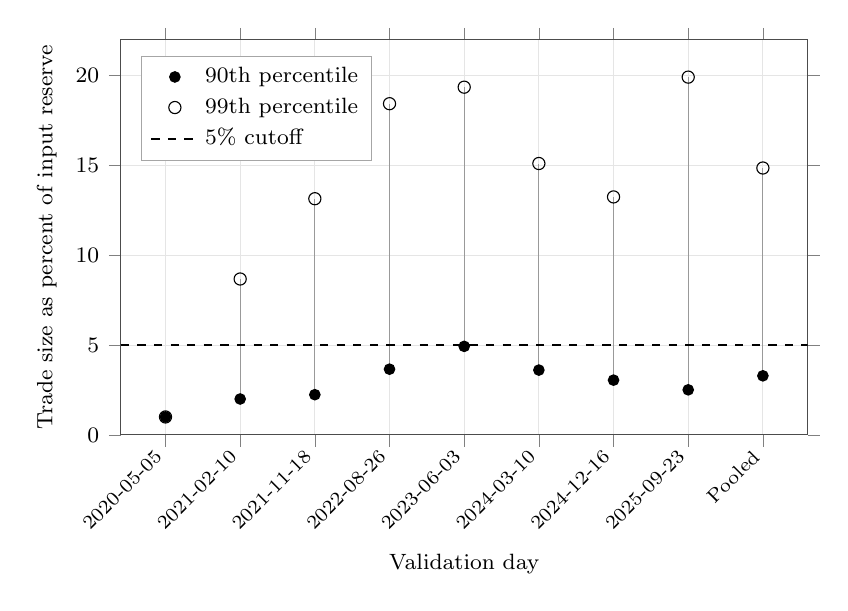
\begin{tikzpicture}
\begin{axis}[width=0.85\textwidth, height=6.6cm, xlabel={Validation day}, ylabel={Trade size as percent of input reserve}, xmin=0.4, xmax=9.6, ymin=0, ymax=22, ytick={0,5,10,15,20}, xtick={1,2,3,4,5,6,7,8,9}, xticklabels={2020-05-05,2021-02-10,2021-11-18,2022-08-26,2023-06-03,2024-03-10,2024-12-16,2025-09-23,Pooled}, x tick label style={rotate=45, anchor=east, font=\scriptsize}, tick align=outside, tick label style={font=\footnotesize}, label style={font=\footnotesize}, legend style={font=\footnotesize, draw=black!35, fill=white, at={(0.03,0.96)}, anchor=north west}, legend cell align=left, grid=major, grid style={black!10}, axis line style={black!70}]
\addplot[black!40, forget plot] coordinates {(1,1.00) (1,1.00)};
\addplot[black!40, forget plot] coordinates {(2,2.00) (2,8.68)};
\addplot[black!40, forget plot] coordinates {(3,2.24) (3,13.15)};
\addplot[black!40, forget plot] coordinates {(4,3.66) (4,18.44)};
\addplot[black!40, forget plot] coordinates {(5,4.93) (5,19.36)};
\addplot[black!40, forget plot] coordinates {(6,3.61) (6,15.11)};
\addplot[black!40, forget plot] coordinates {(7,3.05) (7,13.25)};
\addplot[black!40, forget plot] coordinates {(8,2.51) (8,19.92)};
\addplot[black!40, forget plot] coordinates {(9,3.29) (9,14.86)};
\addplot[only marks, black, mark=*, mark size=1.9pt] coordinates {(1,1.00) (2,2.00) (3,2.24) (4,3.66) (5,4.93) (6,3.61) (7,3.05) (8,2.51) (9,3.29)};
\addlegendentry{90th percentile}
\addplot[only marks, black, mark=o, mark size=2.2pt] coordinates {(1,1.00) (2,8.68) (3,13.15) (4,18.44) (5,19.36) (6,15.11) (7,13.25) (8,19.92) (9,14.86)};
\addlegendentry{99th percentile}
\addplot[black, thick, dashed, no marks] coordinates {(0.4,5) (9.6,5)};
\addlegendentry{5\% cutoff}
\end{axis}
\end{tikzpicture}
\par\vspace{6pt}
\begin{minipage}{0.92\textwidth}
\footnotesize\raggedright \emph{Notes.} The statistic is a leg's input amount as a fraction of the input-side reserve in the pool it would traverse. Points mark the 90th and 99th percentiles; the dashed line marks the 5\% cutoff. The two percentiles coincide on 2020-05-05. The sample contains 932,270 validated swaps on eight dates from 2020-05-05 through 2025-09-23.
\end{minipage}
\end{figure}
% output/exhibits/quoter_support_bounds.jsonl, per-day and pooled 90th and 99th percentiles, 932,270 validated swaps on eight sampled days

This restriction removes economically relevant observations, and the body reports that loss of support. The restriction is calibrated on executed trades, leaving the pricing error of retained hypothetical routes unobserved. A same-block closing-cycle test could provide an indirect check and remains pending.

\section{Markets omitted from the price comparison}
\label{app:coverage}

An omitted venue can improve the best direct route, the best intermediated route, or both. We therefore measure coverage using each venue's share of trading volume and report the composition of the excluded volume. To make volume comparable across the seven data sources, we compute it from individual swaps using the smaller dollar value of the two legs. This avoids double counting in two sources and removes implausible oracle values in thin pools: one Curve pool reports a \$456m day whose swaps sum to \$8, and a constant-product pair with \$255 of reserves reports \$1.36bn. Physical bounds on volume relative to reserves exclude between 0.10\% and 0.24\% of pool-days per year.
% docs/venue-coverage-bounds.md, volume reconstruction, 400 sampled days

\begin{table}[t]
\centering
\caption{Venue shares of panel volume, by year}
\label{tab:app:venues}
\begin{tabular}{lrrrrrrr}
\toprule
Year & Uni v3 & Uni v2 & Curve & Uni v4 & Balancer & Sushi v2 & Sushi v3 \\
\midrule
2020 & 0.00 & 77.51 & 11.36 & 0.00 & 0.00 & 11.13 & 0.00 \\
% docs/venue-coverage-bounds.md, seven-venue shares, sampled days in 2020
2021 & 37.97 & 31.28 & 12.25 & 0.00 & 1.18 & 17.32 & 0.00 \\
% docs/venue-coverage-bounds.md, seven-venue shares, sampled days in 2021
2022 & 64.08 & 7.01 & 18.70 & 0.00 & 5.87 & 4.35 & 0.00 \\
% docs/venue-coverage-bounds.md, seven-venue shares, sampled days in 2022
2023 & 66.81 & 9.26 & 13.88 & 0.00 & 8.80 & 1.22 & 0.03 \\
% docs/venue-coverage-bounds.md, seven-venue shares, sampled days in 2023
2024 & 69.32 & 11.67 & 12.62 & 0.00 & 5.89 & 0.49 & 0.01 \\
% docs/venue-coverage-bounds.md, seven-venue shares, sampled days in 2024
2025 & 60.14 & 4.77 & 10.96 & 22.12 & 1.69 & 0.31 & 0.01 \\
% docs/venue-coverage-bounds.md, seven-venue shares, sampled days in 2025
2026 & 49.35 & 2.43 & 13.52 & 34.24 & 0.16 & 0.12 & 0.18 \\
% docs/venue-coverage-bounds.md, seven-venue shares, sampled days in 2026
\midrule
Pooled & 56.02 & 14.98 & 13.73 & 5.45 & 3.92 & 5.88 & 0.02 \\
% docs/venue-coverage-bounds.md, pooled over all 400 sampled days
\bottomrule
\end{tabular}
\\[4pt]
\footnotesize Percentage shares within the seven-venue panel. Every seventh calendar day from 2018-11-02 to 2026-06-30, 400 sampled days.
\end{table}

Uniswap v4 carries its own within-venue limitation. Pool-identity reconstruction leaves zero swaps with incomplete or invalid immutable pool attributes across 29,005,863 rows. Static-fee pools without hooks account for 84.02\% of swaps and 99.05\% of reported value; the corresponding 2026 shares are 79.89\% and 95.57\%. The excluded remainder uses hooks, dynamic fees, or both, whose transaction-level cash-flow rule is not identified from the raw event.
% output/exhibits/v4_quote_support.jsonl, ALL and 2026 rows by support status

Curve carries between 11\% and 19\% of panel volume in every year it exists and ranks second in four years, making its coverage economically important. The StableSwap model fits 621 pool-days and excludes 588 whose 90th-percentile fitting error exceeds 1\%. Across 28 sampled dates from 2020-02-11 to 2026-04-28, these exclusions account for 34.2\% of the Curve volume assessed, or \$1.83bn of \$5.36bn. Another 2.75\% of Curve volume occurs in pool-days with too few trades to estimate and evaluate the amplification coefficient separately. Lowering the minimum from eight trades to four changes annual excluded shares by at most 1.3 percentage points.
% docs/venue-coverage-bounds.md, 28 measured pool-days from 2020-02-11 to 2026-04-28

\begin{table}[t]
\centering
\caption{Curve volume outside the StableSwap comparison}
\label{tab:app:curveleg}
\small
\begin{tabular}{lrrrrr}
\toprule
\multicolumn{6}{l}{\emph{Panel A: composition of the exclusion}} \\
Leg served & Pool-days & Volume & Of excluded & Of priced & Of that leg \\
\midrule
Native & 374 & \$1.038bn & 56.6\% & 15.7\% & 65.2\% \\
% docs/venue-coverage-bounds.md, 374 excluded Curve pool-days across 28 measured days
Stable & 119 & \$0.752bn & 41.0\% & 79.9\% & 21.1\% \\
% docs/venue-coverage-bounds.md, 119 excluded Curve pool-days across 28 measured days
Other volatile & 95 & \$0.045bn & 2.4\% & 4.4\% & 22.2\% \\
% docs/venue-coverage-bounds.md, 95 excluded Curve pool-days across 28 measured days
\midrule
\multicolumn{6}{l}{\emph{Panel B: excluded share of each leg's volume, by year}} \\
Year & \multicolumn{2}{r}{Native leg} & \multicolumn{2}{r}{Stable leg} & Other volatile \\
\midrule
2021 & \multicolumn{2}{r}{85.49\%} & \multicolumn{2}{r}{46.91\%} & 15.23\% \\
% docs/venue-coverage-bounds.md, Curve pool-days sampled in 2021
2022 & \multicolumn{2}{r}{68.82\%} & \multicolumn{2}{r}{30.21\%} & 50.77\% \\
% docs/venue-coverage-bounds.md, Curve pool-days sampled in 2022
2023 & \multicolumn{2}{r}{59.11\%} & \multicolumn{2}{r}{5.51\%} & 56.60\% \\
% docs/venue-coverage-bounds.md, Curve pool-days sampled in 2023
2024 & \multicolumn{2}{r}{48.24\%} & \multicolumn{2}{r}{0.94\%} & 14.38\% \\
% docs/venue-coverage-bounds.md, Curve pool-days sampled in 2024
2025 & \multicolumn{2}{r}{47.47\%} & \multicolumn{2}{r}{13.96\%} & 10.52\% \\
% docs/venue-coverage-bounds.md, Curve pool-days sampled in 2025
2026 & \multicolumn{2}{r}{60.92\%} & \multicolumn{2}{r}{9.04\%} & 20.08\% \\
% docs/venue-coverage-bounds.md, Curve pool-days sampled in 2026
\bottomrule
\end{tabular}
\\[4pt]
\footnotesize A pool serves the \emph{native} leg when it contains ETH or a staking derivative, the \emph{stable} leg when every token is stable including baskets and interest-bearing wrappers, and the \emph{other volatile} leg otherwise. The sample contains 28 measured Curve pool-days from 2020-02-11 to 2026-04-28. Pool leg is assigned by a token registry pass followed by a symbol pass over stable derivatives, which is required because the registry alone labels metapools pairing a stablecoin against the three-token base-pool claim as volatile pairs.
\end{table}

The exclusions are concentrated in routes involving the native asset. The excluded share of native-leg volume exceeds the stable-leg share by at least 33 percentage points in every sample year and by 54 points in 2023. Tricrypto pools pairing WBTC and WETH with a stablecoin account for \$818m, or 44.6\%, of the \$1.83bn excluded, including seven of the twelve largest excluded pool-days. These pools use CryptoSwap, so the missing coverage is concentrated where Curve supplies depth between ETH and stablecoins.
% docs/venue-coverage-bounds.md, curve_excluded_composition.jsonl, 28 measured pool-days

SushiSwap v3 cannot be priced from the available historical records. Its reserves are distributed across ticks, but the source omits \texttt{sqrtPriceX96}, in-range liquidity, and tick spacing. The balance and weight fields exposed by the common schema do not describe its concentrated-liquidity invariant. This omission is quantitatively small: the venue accounts for 0.016\% of priced-venue volume over the full sample and 0.176\% in 2026. Across fourteen sampled days, only 4.1\% of its volume occurs on token pairs unavailable on another priced venue, never more than \$37,609 on one day.
% docs/venue-coverage-bounds.md, sushiswap_v3_schema_probe.jsonl and sushiswap_v3_pair_overlap.jsonl, 14 sampled days

Balancer accounts for 3.9\% of measured venue volume over the full sample and 8.8\% at its 2023 peak. Weighted pools are included with the validation errors in Table~\ref{tab:app:weighted}. Linear and boosted pools remain outside the comparison. Of 29 sampled composable-stable pools, 23 reduce to two external tokens after removing the pool's own share token, but pricing them also requires historical rate-provider states that are not available in the current source.
% docs/venue-coverage-bounds.md, venue_volume_by_year.jsonl, 400 sampled days; docs/research-workflow.md, Balancer family audit

\section{Round-trip exclusion}
\label{app:roundtrip}

A route whose first input token equals its last output token,
\[
\mathbf{1}\{\,a_{\mathrm{first}} = b_{\mathrm{last}}\,\},
\]
does not represent endpoint-to-endpoint conversion under the paper's route unit. Such routes are removed everywhere before anything is measured because they would otherwise enter a routing statistic as though a trader had chosen an intermediary between distinct endpoints. The excluded population can contain cyclic arbitrage and other self-returning activity; the endpoint rule does not label every route as arbitrage or wash trading. Multi-trade arbitrage can be bundled atomically \citep{DaianEtAl2020FlashBoys}, which supports the mechanism but not an exhaustive behavioural classification.

\begin{table}[t]
\centering
\caption{Round-trip share of multi-leg routing, across 79 sampled days}
\label{tab:app:roundtrip}
\begin{tabular}{lrr}
\toprule
Quantile across days & Share by count & Share by value \\
\midrule
Minimum & 4.45\% & 7.40\% \\
% output/exhibits/round_trip_share_by_day.jsonl, 79 sampled days, minima on 2020-06-01 and 2023-04-03
25th percentile & 9.60\% & 17.73\% \\
% output/exhibits/round_trip_share_by_day.jsonl, 79 sampled days
Median & 12.70\% & 21.72\% \\
% output/exhibits/round_trip_share_by_day.jsonl, 79 sampled days
75th percentile & 17.04\% & 29.56\% \\
% output/exhibits/round_trip_share_by_day.jsonl, 79 sampled days
90th percentile & 20.03\% & 46.11\% \\
% output/exhibits/round_trip_share_by_day.jsonl, 79 sampled days
Maximum & 25.93\% & 91.31\% \\
% output/exhibits/round_trip_share_by_day.jsonl, 79 sampled days, both maxima on 2025-12-06
\midrule
2020 median & 11.77\% & 14.08\% \\
% output/exhibits/round_trip_share_by_day.jsonl, 8 sampled days in 2020
2021 median & 13.21\% & 25.35\% \\
% output/exhibits/round_trip_share_by_day.jsonl, 13 sampled days in 2021
2022 median & 16.72\% & 21.89\% \\
% output/exhibits/round_trip_share_by_day.jsonl, 13 sampled days in 2022
2023 median & 8.51\% & 17.71\% \\
% output/exhibits/round_trip_share_by_day.jsonl, 13 sampled days in 2023
2024 median & 9.60\% & 21.13\% \\
% output/exhibits/round_trip_share_by_day.jsonl, 13 sampled days in 2024
2025 median & 16.75\% & 36.08\% \\
% output/exhibits/round_trip_share_by_day.jsonl, 14 sampled days in 2025
2026 median & 20.80\% & 20.32\% \\
% output/exhibits/round_trip_share_by_day.jsonl, 5 sampled days in 2026
\bottomrule
\end{tabular}
\\[4pt]
\footnotesize Round trips as a share of multi-leg routes. The sample contains 79 dates from 2020-06-01 through 2026-04-27 and 13,160,047 routes, of which 2,488,399 are multi-leg and 351,553 are round trips. Dates with fewer than 200 multi-leg routes are omitted.
\end{table}

The value-weighted share exceeds the count-weighted share at every quantile, by a factor between 1.7 and 3.5, which is consistent with large atomic cycles sitting inside a much larger population of smaller routes. No sampled day is free of them, and the floor of 4.45\% by count falls on 2020-06-01, the earliest day sampled. Count-weighting is used throughout the body because a value-weighted routing statistic on an unscreened panel would give disproportionate influence to this self-returning population. Figure~\ref{fig:app:roundtrip} plots both shares for every sampled day, with the two medians and the extreme day marked.
% output/exhibits/round_trip_share_by_day.jsonl, 79 sampled days from 2020-06-01 to 2026-04-27

\begin{figure}[tbp]
\centering
\caption{Round-trip contamination of multi-leg routing, day by day}
\label{fig:app:roundtrip}
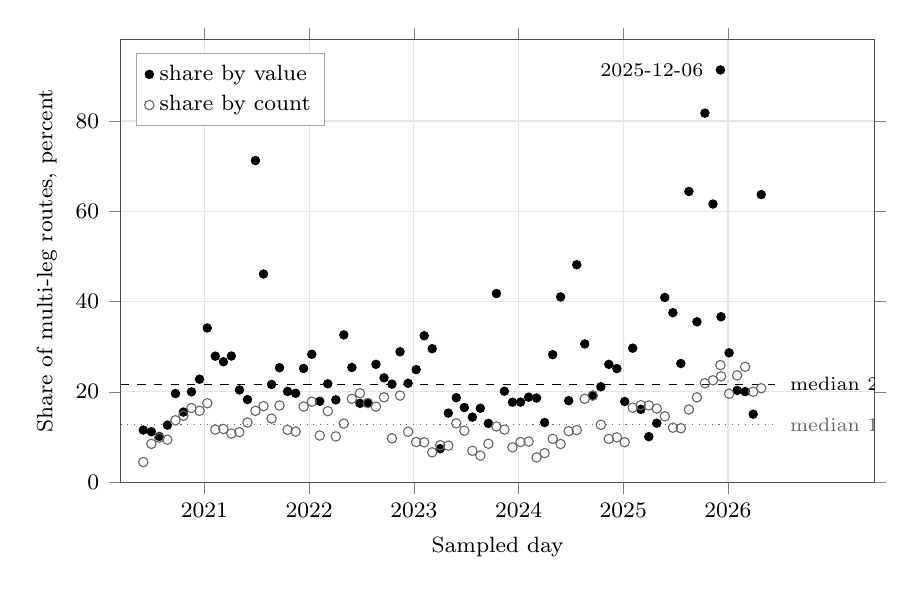
\begin{tikzpicture}
\begin{axis}[width=0.92\textwidth, height=7.2cm, xlabel={Sampled day}, ylabel={Share of multi-leg routes, percent}, xmin=2020.2, xmax=2027.4, ymin=0, ymax=98, xtick={2021,2022,2023,2024,2025,2026}, xticklabel style={/pgf/number format/1000 sep={}}, ytick={0,20,40,60,80}, tick align=outside, tick label style={font=\footnotesize}, label style={font=\footnotesize}, legend style={font=\footnotesize, draw=black!35, fill=white, at={(0.02,0.97)}, anchor=north west}, legend cell align=left, grid=major, grid style={black!10}, axis line style={black!70}]
\addplot[only marks, black, mark=*, mark size=1.5pt] coordinates {(2020.416,11.54) (2020.493,11.17) (2020.569,10.12) (2020.646,12.63) (2020.723,19.62) (2020.799,15.52) (2020.876,20.01) (2020.953,22.80) (2021.027,34.15) (2021.104,27.91) (2021.181,26.67) (2021.257,27.94) (2021.334,20.43) (2021.411,18.29) (2021.487,71.24) (2021.564,46.11) (2021.641,21.64) (2021.717,25.35) (2021.794,20.09) (2021.871,19.68) (2021.947,25.18) (2022.025,28.33) (2022.101,17.92) (2022.178,21.79) (2022.255,18.23) (2022.331,32.62) (2022.408,25.40) (2022.485,17.46) (2022.561,17.57) (2022.638,26.10) (2022.715,23.11) (2022.791,21.72) (2022.868,28.88) (2022.945,21.89) (2023.022,24.93) (2023.099,32.43) (2023.175,29.56) (2023.252,7.40) (2023.329,15.30) (2023.405,18.70) (2023.482,16.53) (2023.559,14.40) (2023.635,16.37) (2023.712,13.02) (2023.789,41.78) (2023.865,20.14) (2023.942,17.71) (2024.019,17.73) (2024.096,18.82) (2024.172,18.63) (2024.249,13.20) (2024.326,28.25) (2024.402,41.03) (2024.479,18.05) (2024.556,48.16) (2024.632,30.62) (2024.709,19.25) (2024.786,21.13) (2024.862,26.10) (2024.939,25.16) (2025.014,17.86) (2025.090,29.68) (2025.167,16.14) (2025.244,10.08) (2025.320,13.06) (2025.397,40.91) (2025.474,37.54) (2025.550,26.28) (2025.627,64.39) (2025.704,35.52) (2025.780,81.75) (2025.857,61.61) (2025.928,91.31) (2025.934,36.64) (2026.011,28.65) (2026.088,20.32) (2026.164,20.06) (2026.241,15.06) (2026.318,63.70)};
\addlegendentry{share by value}
\addplot[only marks, black!60, mark=o, mark size=1.7pt] coordinates {(2020.416,4.45) (2020.493,8.49) (2020.569,9.83) (2020.646,9.41) (2020.723,13.70) (2020.799,14.72) (2020.876,16.42) (2020.953,15.81) (2021.027,17.48) (2021.104,11.64) (2021.181,11.77) (2021.257,10.76) (2021.334,11.07) (2021.411,13.21) (2021.487,15.79) (2021.564,16.84) (2021.641,14.08) (2021.717,16.98) (2021.794,11.57) (2021.871,11.19) (2021.947,16.75) (2022.025,17.82) (2022.101,10.33) (2022.178,15.72) (2022.255,10.13) (2022.331,12.96) (2022.408,18.46) (2022.485,19.69) (2022.561,17.53) (2022.638,16.72) (2022.715,18.80) (2022.791,9.71) (2022.868,19.18) (2022.945,11.17) (2023.022,8.89) (2023.099,8.82) (2023.175,6.60) (2023.252,8.18) (2023.329,8.09) (2023.405,13.02) (2023.482,11.40) (2023.559,6.94) (2023.635,5.88) (2023.712,8.51) (2023.789,12.33) (2023.865,11.64) (2023.942,7.70) (2024.019,8.89) (2024.096,9.00) (2024.172,5.47) (2024.249,6.44) (2024.326,9.60) (2024.402,8.45) (2024.479,11.29) (2024.556,11.53) (2024.632,18.46) (2024.709,19.17) (2024.786,12.70) (2024.862,9.58) (2024.939,9.92) (2025.014,8.85) (2025.090,16.50) (2025.167,17.04) (2025.244,17.00) (2025.320,16.29) (2025.397,14.59) (2025.474,12.06) (2025.550,11.94) (2025.627,16.09) (2025.704,18.79) (2025.780,21.91) (2025.857,22.56) (2025.928,25.93) (2025.934,23.44) (2026.011,19.58) (2026.088,23.65) (2026.164,25.55) (2026.241,20.03) (2026.318,20.80)};
\addlegendentry{share by count}
\addplot[black, dashed, thin, no marks, forget plot] coordinates {(2020.2,21.72) (2026.45,21.72)};
\addplot[black!60, dotted, thin, no marks, forget plot] coordinates {(2020.2,12.70) (2026.45,12.70)};
\node[anchor=west, font=\scriptsize] at (axis cs:2026.5,21.72) {median 21.7};
\node[anchor=west, font=\scriptsize, black!60] at (axis cs:2026.5,12.70) {median 12.7};
\node[anchor=east, font=\scriptsize] at (axis cs:2025.86,91.31) {2025-12-06};
\end{axis}
\end{tikzpicture}
\par\vspace{6pt}
\begin{minipage}{0.92\textwidth}
\footnotesize\raggedright \emph{Notes.} Each mark is one sampled date. \emph{Share by value} weights round-trip routes by their notional; \emph{share by count} gives each route equal weight. Both shares use multi-leg routes as the denominator. Dashed and dotted lines mark the respective medians, and the highest point is labelled. Dates with fewer than 200 multi-leg routes are omitted. The sample contains 79 dates from 2020-06-01 through 2026-04-27 and 2,488,399 multi-leg routes.
\end{minipage}
\end{figure}
% output/exhibits/round_trip_share_by_day.jsonl, share_by_count and share_by_value on 79 sampled days from 2020-06-01 to 2026-04-27


\clearpage

\bibliography{../literature/vehicle-currencies}

\end{document}
